% Options for packages loaded elsewhere
\PassOptionsToPackage{unicode}{hyperref}
\PassOptionsToPackage{hyphens}{url}
%
\documentclass[
  english,
  man,floatsintext]{apa7}
\usepackage{amsmath,amssymb}
\usepackage{lmodern}
\usepackage{ifxetex,ifluatex}
\ifnum 0\ifxetex 1\fi\ifluatex 1\fi=0 % if pdftex
  \usepackage[T1]{fontenc}
  \usepackage[utf8]{inputenc}
  \usepackage{textcomp} % provide euro and other symbols
\else % if luatex or xetex
  \usepackage{unicode-math}
  \defaultfontfeatures{Scale=MatchLowercase}
  \defaultfontfeatures[\rmfamily]{Ligatures=TeX,Scale=1}
\fi
% Use upquote if available, for straight quotes in verbatim environments
\IfFileExists{upquote.sty}{\usepackage{upquote}}{}
\IfFileExists{microtype.sty}{% use microtype if available
  \usepackage[]{microtype}
  \UseMicrotypeSet[protrusion]{basicmath} % disable protrusion for tt fonts
}{}
\makeatletter
\@ifundefined{KOMAClassName}{% if non-KOMA class
  \IfFileExists{parskip.sty}{%
    \usepackage{parskip}
  }{% else
    \setlength{\parindent}{0pt}
    \setlength{\parskip}{6pt plus 2pt minus 1pt}}
}{% if KOMA class
  \KOMAoptions{parskip=half}}
\makeatother
\usepackage{xcolor}
\IfFileExists{xurl.sty}{\usepackage{xurl}}{} % add URL line breaks if available
\IfFileExists{bookmark.sty}{\usepackage{bookmark}}{\usepackage{hyperref}}
\hypersetup{
  pdftitle={The validity of the self-compassion scale: A study on post-traumatic growth and post-traumatic stress symptoms in a sample of rescue workers},
  pdfauthor={Corrado Caudek1, Claudio Sica2, Celeste Berti1, Ilaria Colpizzi1, \& Virginia Alfei1},
  pdflang={en-EN},
  pdfkeywords={self-compassion; rescue workers; Self-compassion Scale (SCS); post-traumatic growth; post-traumatic stress; neuroticism; structural equation modelling; latent profile analysis},
  hidelinks,
  pdfcreator={LaTeX via pandoc}}
\urlstyle{same} % disable monospaced font for URLs
\usepackage{graphicx}
\makeatletter
\def\maxwidth{\ifdim\Gin@nat@width>\linewidth\linewidth\else\Gin@nat@width\fi}
\def\maxheight{\ifdim\Gin@nat@height>\textheight\textheight\else\Gin@nat@height\fi}
\makeatother
% Scale images if necessary, so that they will not overflow the page
% margins by default, and it is still possible to overwrite the defaults
% using explicit options in \includegraphics[width, height, ...]{}
\setkeys{Gin}{width=\maxwidth,height=\maxheight,keepaspectratio}
% Set default figure placement to htbp
\makeatletter
\def\fps@figure{htbp}
\makeatother
\setlength{\emergencystretch}{3em} % prevent overfull lines
\providecommand{\tightlist}{%
  \setlength{\itemsep}{0pt}\setlength{\parskip}{0pt}}
\setcounter{secnumdepth}{-\maxdimen} % remove section numbering
% Make \paragraph and \subparagraph free-standing
\ifx\paragraph\undefined\else
  \let\oldparagraph\paragraph
  \renewcommand{\paragraph}[1]{\oldparagraph{#1}\mbox{}}
\fi
\ifx\subparagraph\undefined\else
  \let\oldsubparagraph\subparagraph
  \renewcommand{\subparagraph}[1]{\oldsubparagraph{#1}\mbox{}}
\fi
% Manuscript styling
\usepackage{upgreek}
\captionsetup{font=singlespacing,justification=justified}

% Table formatting
\usepackage{longtable}
\usepackage{lscape}
% \usepackage[counterclockwise]{rotating}   % Landscape page setup for large tables
\usepackage{multirow}		% Table styling
\usepackage{tabularx}		% Control Column width
\usepackage[flushleft]{threeparttable}	% Allows for three part tables with a specified notes section
\usepackage{threeparttablex}            % Lets threeparttable work with longtable

% Create new environments so endfloat can handle them
% \newenvironment{ltable}
%   {\begin{landscape}\begin{center}\begin{threeparttable}}
%   {\end{threeparttable}\end{center}\end{landscape}}
\newenvironment{lltable}{\begin{landscape}\begin{center}\begin{ThreePartTable}}{\end{ThreePartTable}\end{center}\end{landscape}}

% Enables adjusting longtable caption width to table width
% Solution found at http://golatex.de/longtable-mit-caption-so-breit-wie-die-tabelle-t15767.html
\makeatletter
\newcommand\LastLTentrywidth{1em}
\newlength\longtablewidth
\setlength{\longtablewidth}{1in}
\newcommand{\getlongtablewidth}{\begingroup \ifcsname LT@\roman{LT@tables}\endcsname \global\longtablewidth=0pt \renewcommand{\LT@entry}[2]{\global\advance\longtablewidth by ##2\relax\gdef\LastLTentrywidth{##2}}\@nameuse{LT@\roman{LT@tables}} \fi \endgroup}

% \setlength{\parindent}{0.5in}
% \setlength{\parskip}{0pt plus 0pt minus 0pt}

% Overwrite redefinition of paragraph and subparagraph by the default LaTeX template
% See https://github.com/crsh/papaja/issues/292
\makeatletter
\renewcommand{\paragraph}{\@startsection{paragraph}{4}{\parindent}%
  {0\baselineskip \@plus 0.2ex \@minus 0.2ex}%
  {-1em}%
  {\normalfont\normalsize\bfseries\itshape\typesectitle}}

\renewcommand{\subparagraph}[1]{\@startsection{subparagraph}{5}{1em}%
  {0\baselineskip \@plus 0.2ex \@minus 0.2ex}%
  {-\z@\relax}%
  {\normalfont\normalsize\itshape\hspace{\parindent}{#1}\textit{\addperi}}{\relax}}
\makeatother

% \usepackage{etoolbox}
\makeatletter
\patchcmd{\HyOrg@maketitle}
  {\section{\normalfont\normalsize\abstractname}}
  {\section*{\normalfont\normalsize\abstractname}}
  {}{\typeout{Failed to patch abstract.}}
\patchcmd{\HyOrg@maketitle}
  {\section{\protect\normalfont{\@title}}}
  {\section*{\protect\normalfont{\@title}}}
  {}{\typeout{Failed to patch title.}}
\makeatother
\shorttitle{Mapping the nomological network of the SCS}
\keywords{self-compassion; rescue workers; Self-compassion Scale (SCS); post-traumatic growth; post-traumatic stress; neuroticism; structural equation modelling; latent profile analysis\newline\indent Word count: 6511}
\usepackage{csquotes}
\usepackage{rotating}
\DeclareDelayedFloatFlavor{sidewaysfigure}{figure}
\DeclareDelayedFloatFlavor{sidewaystable}{table}
\usepackage{pdflscape}
\DeclareDelayedFloatFlavor{landscape}{table}
\raggedbottom
\usepackage{xcolor,makecell,array}
\usepackage{graphicx}
\setlength{\parskip}{0pt plus 0pt minus 0pt}
\usepackage{multirow}
\usepackage{setspace}
\usepackage{booktabs}
\usepackage{tabularx}
\usepackage{caption}
\usepackage{color, colortbl}
\usepackage{newfloat}
\usepackage{glossaries}
\makeglossaries
\DeclareFloatingEnvironment[fileext=los, listname=List of Schemes, name=Listing, placement=!htbp, within=section]{listing}
\usepackage{placeins}
\ifxetex
  % Load polyglossia as late as possible: uses bidi with RTL langages (e.g. Hebrew, Arabic)
  \usepackage{polyglossia}
  \setmainlanguage[]{english}
\else
  \usepackage[main=english]{babel}
% get rid of language-specific shorthands (see #6817):
\let\LanguageShortHands\languageshorthands
\def\languageshorthands#1{}
\fi
\ifluatex
  \usepackage{selnolig}  % disable illegal ligatures
\fi
\newlength{\cslhangindent}
\setlength{\cslhangindent}{1.5em}
\newlength{\csllabelwidth}
\setlength{\csllabelwidth}{3em}
\newenvironment{CSLReferences}[2] % #1 hanging-ident, #2 entry spacing
 {% don't indent paragraphs
  \setlength{\parindent}{0pt}
  % turn on hanging indent if param 1 is 1
  \ifodd #1 \everypar{\setlength{\hangindent}{\cslhangindent}}\ignorespaces\fi
  % set entry spacing
  \ifnum #2 > 0
  \setlength{\parskip}{#2\baselineskip}
  \fi
 }%
 {}
\usepackage{calc}
\newcommand{\CSLBlock}[1]{#1\hfill\break}
\newcommand{\CSLLeftMargin}[1]{\parbox[t]{\csllabelwidth}{#1}}
\newcommand{\CSLRightInline}[1]{\parbox[t]{\linewidth - \csllabelwidth}{#1}\break}
\newcommand{\CSLIndent}[1]{\hspace{\cslhangindent}#1}

\title{The validity of the self-compassion scale: A study on post-traumatic growth and post-traumatic stress symptoms in a sample of rescue workers}
\author{Corrado Caudek\textsuperscript{1}, Claudio Sica\textsuperscript{2}, Celeste Berti\textsuperscript{1}, Ilaria Colpizzi\textsuperscript{1}, \& Virginia Alfei\textsuperscript{1}}
\date{}


\authornote{

\addORCIDlink{Corrado Caudek}{0000-0002-1404-0420}

Add complete departmental affiliations for each author here. Each new line herein must be indented, like this line.
Enter author note here.

Correspondence concerning this article should be addressed to Corrado Caudek, NEUROFARBA Department, Psychology Section, University of Firenze, Italy. E-mail: \href{mailto:corrado.caudek@unifi.it}{\nolinkurl{corrado.caudek@unifi.it}}

}

\affiliation{\vspace{0.5cm}\textsuperscript{1} NEUROFARBA Department, Psychology Section, University of Florence, Italy\\\textsuperscript{2} Health Sciences Department, Psychology Section, University of Florence, Italy}

\abstract{
It is debated whether self-compassion (a constructs from within the Buddhist psychology) should be understood as a ``holistic'' construct, or as a two-factor structure corresponding to the positively phrased items (self-kindness, common humanity, mindfulness) and the negatively phrased items (self-judgment, isolation, over-identification) of the Self-Compassion Scale (SCS; Neff, 2003). Here, we examined a sample of rescue workers who manifest greater compassionate responding (CS) and reduced uncompassionate responding (RUS) than traditional community and student samples. The factor structure of the SCS was studied by examing the relations among self-compassion, coping, perceived social support, neuroticism, post-traumatic stress (PTS), and post-traumatic growth (PTG). Through structural equation modeling (SEM), we found that a two-factor characterization (CS vs RUS) of the SCS provided a better fit to the nomological network including the above mentioned variables, rather than a one-factor characterization of the SCS. We also found that the CS and RUS components of self-compassion had a different functional role when considering their effects on PTS and PTG. These results differ from those of previous studies because the relation of self-compassion to adaptive/disadaptive psychological functioning is context specific. The present results strengthen the idea that CS and RUS are functionally different components of self-compassion.
}



\begin{document}
\maketitle

\hypertarget{introduction}{%
\section{Introduction}\label{introduction}}

A growing interest has been recently directed to the concept of the ``self'' as a relevant construct for advancing our understanding of individual differences in relation to coping and stress (Beck, 2016). Specific ways of interacting with the self, which can be described with constructs from within the Buddhist psychology, such as self-compassion (SC), have been shown to be beneficial for mental health (MacBeth \& Gumley, 2012). In particular, a compassionate mindset towards oneself has been proposed as a protective factor against psychopathology, including Post-Traumatic Stress Disorder {[}PTSD; Kirby et al. (2017); Wilson et al. (2019){]}, and as a factor promoting a positive change that is sometimes experienced by individuals dealing with traumatic events, which is known as Post-Traumatic Growth {[}PTG; Wong and Yeung (2017){]}.

Self compassion has emerged as a protective factor against PTSD because it has been shown to be associated (1) with easing the negative impact of trauma and PTSD symptoms (Janoff-Bulman, 1989), (2) with lower levels of shame, which is a form of internal threat following trauma (Keene \& Epps, 2016), (3) with adaptive coping strategies (Seligowski et al., 2015), (4) with improved emotional regulation (Badour \& Feldner, 2013), resilience (Seligowski et al., 2015), and a greater ability to manage distress (Barlow et al., 2017), (5) and with feeling interpersonally connected to others (Aspy \& Proeve, 2017), which is a trauma-resilience factor (Bistricky et al., 2017) -- for a recent review, see Winders et al. (2020).

Self compassion has also been shown to lead to PTG, that is, to positive changes that follow a traumatic event and bring about changes in self-perception, in interpersonal relationships, and in a reevaluation of one's own view of the world (Tedeschi \& Calhoun, 2004). Such positive changes take place by reducing ruminations and depressive symptoms (Nolen-Hoeksema et al., 2008) and by providing a more effective coping strategy with stress through reliance on positive cognitive restructuring (Allen \& Leary, 2010). For example, Wong and Yeung (2017) showed that the relation between self-compassion and PTG is mediated by several adaptive cognitive processes such as acceptance, positive reframing and presence of meaning. Moreover, Chishima et al. (2018) found that high self-compassion participants tended to judge stressful events as less threatening and more controllable than low self-compassion participants.

Despite the enormous interest in self-compassion in recent years, and despite the plethora of studies that have examined self-compassion in relation to PTSD and PTG, the usefulness of the self-compassion construct in relation to psychopathology has been strongly challenged (\emph{e.g.}, Muris et al., 2021). The purpose of the present study is to contribute to this debate by examining the relation between self-compassion, PTSD, and PTG in a sample of rescue workers, that is, in a context in which the effects of self-compassion on the other two constructs may be more evident than in community or student samples that have been typically examined in previous studies.

\hypertarget{the-self-compassion-scale}{%
\subsection{The Self-Compassion Scale}\label{the-self-compassion-scale}}

Self-compassion is commonly assessed with the Self-Compassion Scale (SCS), a 26 item self-report scale which spans six dimensions of the construct (Neff, 2003b). Three sub-sets of items are considered indicators of Compassionate Self-responding (CS): (a) being kind and understanding toward one's fallibility, (b) acknowledging that personal failures and pain are something that everyone experiences, and (c) having a mindful awareness of one's painful thoughts and feelings. The remaining three sub-sets of items are considered indicators of Reduced Uncompassionate Self-responding (RUS): (a) being critical and not understanding toward personal shortcomings, (b) having the tendency of isolating from others, and (c) avoiding one's painful thoughts and feelings or overidentifying with them (Muris \& Otgaar, 2020). The SCS total score is given by the sum of the self-responding on the compassionate items and the reversely scored uncompassionate items.

Although the SCS has been extremely popular in the recent psychological literature (for a recent review, see Muris \& Otgaar, 2020), questions have been raised about its validity as a measure of self-compassion (Kandler et al., 2017; Muris, 2016; Muris et al., 2016, 2019; Muris \& Petrocchi, 2017). It has been pointed out that, rather than presenting a more nuanced picture of this construct, by means of the SCS self-compassion is understood as a ``pure protective factor'' (\emph{e.g.}, Gu et al., 2020; Montero-Marin et al., 2018; Seppälä et al., 2017; Strauss et al., 2016). This depend on the fact that the data of the SCS are (usually) summarized in terms of the SCS total score. However, this choice is problematic for several reasons (Muris \& Otgaar, 2020).

\begin{enumerate}
\def\labelenumi{\arabic{enumi}.}
\item
  The SCS total score might inflate the link with psychopathology, given that the relations found between the SCS total scores and other psychological constructs might mainly depend on the RUS component of the SCS (Muris et al., 2018). The RUS component of the SCS is strongly associated with symptoms such as anxiety and depression (Muris \& Petrocchi, 2017) and, once RUS is removed from the SCS, the added value of CS might be marginal (Muris et al., 2019).
\item
  Some scholars have cast doubt on the central component of the SCS (\emph{i.e.}, CS) by arguing that CS may be redundant, because it overlaps with with the personality trait of Neuroticism: Once Neuroticism is controlled, there is no evidence of a specific contribution of compassionate self-responding (Geiger et al., 2018; Kandler et al., 2017).
\item
  Lastly, it has been suggested that the common use of the SCS total score may obscure the associations that may be found in therapeutic interventions between treatment effects and the putative components of the SCS (Wadsworth et al., 2018).
\end{enumerate}

One limit of previous studies on the SCS was that they mostly included community or student populations, that is, they examined situations in which PTSD and PTG were only present in mild forms. The purpose of the present study is to evaluate the hypotheses of Muris et al. (2019) and of Geiger et al. (2018) in a sample of rescue workers, where the individual differences in adaptive or maladaptive responses to stress are expected to be stronger than in community or student samples.

\hypertarget{self-compassion-ptsd-and-ptg-in-rescue-workers}{%
\subsection{Self-compassion, PTSD, and PTG in rescue workers}\label{self-compassion-ptsd-and-ptg-in-rescue-workers}}

Rescue workers are first responders to traumatic event such as earthquakes, geological disasters, fire, meteorological disasters, and are involved in acute health crises, such as the current pandemic. They engage in out-of-hospital acute medical care, contribute to transportation to definitive care, or provide assistance during disasters and life-threatening conditions in a professional or voluntary capacity (Berger et al., 2012). The high exposure to traumatic events of rescue workers, as part of their professional practice, often comes at a personal cost, resulting in psychological problems such as depression, anxiety, and PTSD at a much higher prevalence than the general public (\emph{e.g.}, Palgi et al., 2009; Witteveen et al., 2007). Psychological factors can exacerbate or ameliorate the consequences of such exposure to trauma: It has been shown that a personal history of negative life events increases the likelihood of negative consequences accompanying the hardships of caring for victims, whereas other factors, including compassion satisfaction {[}\emph{i.e.}, the positive experiences deriving from being able to help others; Sodeke-Gregson et al. (2013){]}, may act as protection (Adams et al., 2006).
In the present study, we will use a sample of rescue workers to examine some of the outstanding questions that have been raised in the previous literature concerning the validity of the SCS (Neff, 2003a).

\hypertarget{aims-of-the-study}{%
\section{Aims of the study}\label{aims-of-the-study}}

\begin{itemize}
\item
  \textbf{Question Q1}: It has been proposed that the relations of the SCS (Neff, 2003a) with psychopathology are only due to the negative component of SC, with the effects of the positive component of SC being negligible (Muris et al., 2019). Here, we examine the factor structure of the SCS in the context of a nomological network including PTSD and PTG. We ask whether the associations between these constructs are better described by using the SCS total score, or by distinguishing between the CS and RUS components of the SCS (Muris et al., 2021; Muris \& Otgaar, 2020; \emph{e.g.}, Neff et al., 2019).
\item
  \textbf{Question Q2}: Previous studies on self-compassion have focused, for the most part, on a population which is not normally exposed to events leading to PTG or PTS (\emph{i.e.}, undergraduate students). Here, we examine the possibility that self-compassion may be experienced differently by individuals with different levels of exposure to traumatic events.
\item
  \textbf{Question Q3}: The validity of the SCS has been challenged by arguing that self compassion reduces to Neuroticism (Geiger et al., 2018). To evaluate this claim, we examine the added value that can be attributed to self-compassion in a nomological network that includes Neuroticism, PTG, and PTS.
\end{itemize}

\hypertarget{methods}{%
\section{Methods}\label{methods}}

\hypertarget{participants}{%
\subsection{Participants}\label{participants}}

A call for the participation in the study was advertised in the Italian Red Cross websites of Lombardy and Tuscany. This resulted in a sample of \emph{n} = 783 participating emergency (first-time responders) rescue-workers (46\% female) with 8.77 (8.08) mean years of experience as rescue worker, and in a sample of \emph{n} = 324 students and community participants (74\% female). Mean age was 41.1 (\emph{SD} = 13.9) and 25.6 (10.8) years for rescue workers and controls, respectively. For rescue-workers, mean rate of activity was 0.94 (0.58) times per week.

\hypertarget{material}{%
\subsection{Material}\label{material}}

Specific questions for ambulance personnel were developed to investigate the rescue-workers' role (such as driver, team leader, rescuer, etc.), number of weekly shifts, and number of psychological support meeting (such as debriefing and defusing). Moreover, participants were asked whether they had experienced traumatic events in their lives.

The \emph{Post-Traumatic Growth Inventory} {[}PTGI; Tedeschi and Calhoun (1996){]} is a 21 item self-report measure.
PTGI evaluates the growth following one or more stressful or traumatic events in one's life. The PTGI comprises five sub-scales (Relation with others, New possibilities, Personal strength, Appreciation of life, and Spiritual changes) and has good internal consistency, construct-convergent validity, and discriminant validity (Tedeschi \& Calhoun, 1996). Also the Italian version has good internal consistency and validity (Prati \& Pietrantoni, 2014).
In the present sample, each sub-scale show good-to-excellent Chronbach's \(\alpha\) values: Relation with others = 0.94, New possibilities = 0.91, Personal strength = 0.86, Appreciation of life = 0.85, Spiritual changes = 0.89; total = 0.97.

The \emph{Impact of Event Scale - Revised} {[}IES-R; Weiss (2007){]} is a 22-item self-report measure assessing subjective distress caused by traumatic events and it is based on the views of the core phenomena of traumatic-stress reactions: intrusion (B criteria in the DSM-IV PTSD diagnosis), avoidance (C criteria), and persistent hyper-arousal. Correspondingly, the IES-R comprises the sub-scales of Intrusion, Avoidance, and Hyper-arousal. The IES-R is widely used to assess the symptomatology of the PTSD in rescue workers. The IES-R show good internal consistency and test--retest stability. The Italian translation show good psychometric properties, good concurrent and discriminant validity, and good test--retest reliability (Craparo et al., 2013). In the present sample, each sub-scale show good-to-excellent Chronbach's \(\alpha\) values: Intrusion = 0.93, Avoidance = 0.86, Hyperarousal = 0.91; total = 0.96.

The \emph{Multi-dimensional Scale of Perceived Social Support} {[}MSPSS; Zimet et al. (1988){]}, a 12 items self-report questionnaire, was used to assess the perceived adequacy of social support from from family members, friends, and significant others. We used the Italian version of the MSPSS. The original version of the MSPSS has very good internal reliability properties for the three sub-scales (Zimet et al., 1990). The Italian version show good internal consistency, test--retest reliability (Fabio \& Kenny, 2012), and validity (Prezza \& Giuseppina Pacilli, 2002). In the present sample, the three sub-scales show excellent Chronbach's \(\alpha\) values: Family = 0.96, Friends = 0.97, Significant Others = 0.96; total = 0.95.

The \emph{NEO-Five Factor Inventory} (NEO-FFI-60; Costa and McCrae (1992)), a 60 items self-report questionnaire, was used to assess five broad domains of personality: Neuroticism (N), Extraversion (E), Openness to experience (O), Agreeableness (A), and Conscientiousness (C). The internal consistency of the five sub-scales of the NEO-FFI-60 is adequate (Murray et al., 2003). In the present sample, the Italian version by Caprara et al. (2001), produce the following Chronbach's \(\alpha\) values: N = 0.89, E = 0.83, O = 0.72; A = 0.73, C = 0.88; total = 0.77. In the present study, only the Neuroticism sub-scale was used.

The \emph{Coping Orientation to Problems Experienced} test (COPE; Carver et al. (1989){]}, a 60 items self-report questionnaire, was used to evaluate the skills and strategies adopted to face stressful and difficult events. The COPE comprises five dimensions (social support, avoidance strategies, positive attitude, problem-solving, and transcendent orientation) and has adequate internal consistency, and convergent and discriminant validity (Carver et al., 1989).
Factor analyses on the Italian version of the COPE {[}Sica et al. (1997); Sica et al. (2008); sica2021facing{]} have demonstrated that the scales can be grouped into the following dimensions: Problem-focused, Social Support, Avoidance-oriented, Positive-oriented, and Transcendent-oriented. Internal consistency values of these five dimensions in the present sample exceeded 0.80, with the exception of the Avoidance-oriented coping (Cronbach's \(\alpha\) = 0.75). In the present sample, internal consistency values for the Italian version are the following: Social support = 0.91, Avoidance strategies 0 =.87, Positive attitude = 0.79, Problem-solving = 0.87, Transcendent orientation = 0.82; total = 0.86. In the present study, only the Positive\_attitude and Problem solving sub-scales were used.
\emph{Self-Compassion Scale} {[}SCS; Neff (2003a); Italian version by Veneziani et al. (2017){]}, a 26 items self-report questionnaire, was used to evaluate self-compassion. High levels of self-compassion reflect an ability to be kind and understanding toward oneself, even in difficult times. The psychometric properties of the SCS in the present sample are discussed in the Results section.

\hypertarget{data-analysis-plan}{%
\subsection{Data analysis plan}\label{data-analysis-plan}}

To answer Question Q1 (\emph{i.e.}, what is the dimensionality of the SCS?), we performed confirmatory factor analysis (CFA). Several factor structures were compared and goodness‐of‐fit was evaluated according to the Comparative Fit Index (CFI), Tucker-Lewis Index (TLI), Root Mean Square Error Approximation (RMSEA), and Standardized Root Mean Square Residual (SRMR). In order to avoid falsely rejecting viable latent variable models, the following cut-off criteria were used: RMSEA and SRMR near or less than 0.08, and CFI and TLI near or greater than 0.90 (Little, 2013; West et al., 2012). A weighted least squares mean- and variance-adjusted estimator (WLSMV) was used to assess each latent construct, as it is more adequate than maximum-likelihood for ordered-categorical items with five or less response options (\emph{e.g.}, Bandalos, 2014). To study the dimensionality of the SCS, we used both traditional CFA models and Exploratory Structural Equation Modeling {[}ESEM; Asparouhov and Muthén (2009){]}. The ESEM strategy is used for modeling multidimensional constructs comprising a certain overlap between the hypothesized theoretical dimensions. In such circumstances, ESEM overcomes the limitation stemming from the fact that the zero cross-loading specification assumed by traditional CFA can be too rigid (see also Neff et al., 2019). To further validate the bidimensional structure of the SCS, CFA and ESEM modeling was complemented by Latent Profiles Analysis (LPA). LPA is a person-centered modeling approach aiming at identifying subgroups of participants based on patterns of characteristics assessed within a study. Specifically, we compared the groups recovered by LPA, which were identified in terms of the CS and RUS components of the SCS, according to their PTG and PTSD scores. In this context, we examined two extreme hypotheses: The first assumes that CS is related to PTG but not to PTSD, and that RUS is related to PTSD but not to PTG; the second assumes the opposite (\emph{i.e.}, RUS is related to PTG but not to PTSD; CS is related to PTSD but not to PTG). If CS and RUS are equivalent measures of the self-compassion construct, then both hypotheses should be confirmed. Conversely, if CS and RUS represent distinct dimensions of the self-compassion construct, then only the first hypothesis should be accepted.

To answer Question Q2 (\emph{i.e.}, does self-compassion vary across groups with different levels of exposure to traumatic events?), we compared the SCS total score, CS, and RUS across rescue workers and a control group, when also considering age and gender. If the results showed group differences articulated in terms of CS and RUS, or different interactions between group and age or gender when considering CS or RUS, we would conclude that is not meaningful to operationalize self-compassion in terms of the SCS total score.

To answer Question Q3 (\emph{i.e.}, does the CS component of the SCS reduce to neuroticism?), we compared several Structural Equations Models (SEMs) examining self-compassion within a larger nomological network which comprised PTG, PTSD, coping, and neuroticism.

Nested models were compared by using the \(\chi^2\)-difference test and not nested model were compared by several fit indices: decreases in the CFI and TLI more than .01 and increases in the RMSEA more than .015 (Chen, 2007; Cheung \& Rensvold, 2002). All CFA and SEM models were tested using Mplus version 8.6 (B. Muthén \& Muthén, 2017) using all available data. For ordinal measures, the robust weighted least squares (mean and variance adjusted)-procedure (WLSMV) was used for parameter estimation and assessing model fit (B. O. Muthén et al., 2015).

\hypertarget{results}{%
\section{Results}\label{results}}

\hypertarget{preliminary-analysis-and-descriptive-statistics}{%
\subsection{Preliminary analysis and descriptive statistics}\label{preliminary-analysis-and-descriptive-statistics}}

The traumatic events that were experienced by the rescue-workers during their activity fell more often into one of the following categories: cardiorespiratory arrest (36\%), major trauma (25\%), suicide (10\%), domestic violence (6\%), intervention for cardiac arrest on a minor (4\%), child maltreatment (3\%), car accident (2\%).
Major life events experienced by the rescue-workers fell more often into one of the following categories: death of a first-degree relative including a child or spouse (45\%), serious illness or injury to the subject (17\%), becoming unemployed or seeking work for more than one month (7\%), a major financial crisis (5\%), separation due to marital difficulties (5\%), serious problems with a close friend, neighbor or relative (4\%), being sacked from one's job, (4\%), serious illness or injury to a close relative (2\%), breaking off a steady relationship (1\%).

The mean total score on the IES-R was 17.76 (\emph{SD} = 15.75). By using a cut-off of 33 on the IES-R total score (Creamer et al., 2003), 135 (17\%) rescue workers participants were identified as probable PTSS cases; of them, 60\% were women. For rescue workers, average PTG was 39.21 (24.65). IES-R and PTG data were not collected for controls.

\hypertarget{q1-dimensionality-of-the-scs}{%
\subsection{Q1: Dimensionality of the SCS}\label{q1-dimensionality-of-the-scs}}

\hypertarget{scs-factor-structure}{%
\subsubsection{SCS factor structure}\label{scs-factor-structure}}

To examine the factor structure of the SCS (Muris et al., 2021; Muris \& Otgaar, 2020; \emph{e.g.}, Neff et al., 2019), all items from the Self-judgment, Isolation, and Over-identification subscales of the SCS were reverse‐coded before analyses. In a set of preliminary analyses, we tested all factor-structure models described by Neff et al. (2019) (see Supplementary Materials). Consistent with Neff et al. (2019), the bifactor ESEM models -- Models 4b and 5b in Neff et al. (2019) -- were found to provide the best description of the factor structure of the SCS. Such models are closer to the view that self-compassion is comprised of six components that interact as a global system, as proposed by Neff (2003a). We then considered three further factor models not discussed by Neff et al. (2019).

\begin{enumerate}
\def\labelenumi{\arabic{enumi}.}
\item
  A bifactor two-factor ESEM model, with correlated SC and RUS factors. This model identifies an ESEM CS factor with 13 target items (\emph{i.e.}, the items for self-kindness, common humanity, and mindfulness) and a RUS factor with 13 target items (\emph{i.e.}, the items for reduced self-judgment, reduced isolation, and reduced over-identification). The correlation between the CS and RUS factors was -0.190. A further general factor, uncorrelated with CS and RUS, saturated on all indicators. The fit indices were the following: CFI = 0.92, TLI = 0.89, RMSEA = 0.09 {[}90\% CI 0.09-0.10{]}, SRMR = 0.04, \(\omega_t\) = 0.96.
\item
  Given that the previous model approximated psychometric adequacy, we examined its modification indices. The modification indices of the previous model suggested allowing residual correlations between items SCCH10 (``When I feel inadequate in some way, I try to remind myself that feelings of inadequacy are shared by most people'') and SCCH7 (``When I'm down and out, I remind myself that there are lots of other people in the world feeling like I am''), and between items SCIS18 (``When I'm really struggling, I tend to feel like other people must be having an easier time of it'') and SCIS13 (``When I'm feeling down, I tend to feel like most other people are probably happier than I am'').
  Although allowing correlated indicator residuals is generally inappropriate, this issue may be in part alleviated by considering the strong content similarity of the two pairs of indicators listed above (\emph{e.g.}, Siefert et al., 2020).
  With this change, quality of fit was acceptable: CFI = 0.95, TLI = 0.93, RMSEA = 0.08 {[}90\% CI 0.07-0.08{]}, SRMR = 0.03, \(\omega_t\) = 0.96.
  The correlation between the SC and RUS factors was -0.207; \(r_{\text{10, 7}}\) = 0.340; \(r_{\text{18, 13}}\) = 0.223.
\item
  A two-factor ESEM model for the correlated CS and RUS factors. Although this model was already examined by Neff et al. (2019), we used a different factor extraction procedure -- see Supplementary Material.
  Also this model showed an adequate fit of our data: CFI = 0.93, TLI = 0.93, RMSEA = 0.07 {[}90\% CI 0.07-0.08{]}, SRMR = 0.07, \(\omega_t\) = 0.95.
  The correlation between the CS and RUS factors was -0.277.
\end{enumerate}

In summary, two measurement models with two separate factors for the CS and RUS components met our criteria for at least adequate fit. Although the ``holistic'' bifactor ESEM model with six specific factors (which supports the use of the SCS total score) showed slightly better goodness of fit indices, the two factor model (which supports the differential coding of the CS and RUS components) showed sufficient psychometric adequacy to warrant its use in further statistical analyses.

\hypertarget{latent-profiles-analysis}{%
\subsubsection{Latent Profiles Analysis}\label{latent-profiles-analysis}}

A further test of the two-dimensional nature of self-compassion was carried out by means of a Latent Profiles Analysis (LPA). LPA allows to identify underlying latent sub-groups, or profiles, based on common response patterns. Prior to the analysis, the six self-compassion dimensions were standardized and scores on the three RUS sub-scales were reversed (\emph{i.e.}, they were considered as indicators of ``lack of'' Self judgment, Overidentification, and Isolation). For the present data, the best LPA solution was a model with 6 classes (see Ullrich-French \& Cox, 2020) -- see Fig.~\ref{fig:figureLPA} for a description of the obtained profiles.

A first result is that the LPA solution identified self-compassion profiles that clearly reflect the distinction between the CS and RUS dimensions {[}\emph{i.e.}, groups differing in terms of self-compassionate, reduced uncompassionate, and average (moderate) scores{]}. These dimensional patterns are consistent with Neff's description of responses that mirror the inverse relationships between the negative and positive dimensions of self-compassion, and support the ides that self-compassion is best represented in terms of a description comprising two-dimensional scores (see also Phillips, 2019; Ullrich-French \& Cox, 2020).

To validate the LPA solution and, implicitly, the two-dimensional characterization of self-compassion, we related the groups identified by LPA with two external dimensions: IES-R and PTG. We contrasted two alternative hypotheses. \textbf{H1:} CS and RUS have functionally different purposes: CS promotes adaptive responses (operationalized in terms of PTG scores), whereas RUS prevents maladaptive responses (operationalized in terms of IES-R scores). \textbf{H2:} the CS and RUS components have the same functional purpose (\emph{i.e.}, they are related in the similar manner to PTG and IES-R); H2 is thus consistent with the ``holistic'' characterization of the SCS structure. H1 predicts, for example, higher PTG scores in a profile with high CS levels and low RUS levels than in a profile with low CS levels and high RUS levels. For the same two profiles, conversely, H1 predicts lower IES-R scores in a profile with high CS levels and low RUS levels than in a profile with low CS levels and high RUS levels.

To contrast these two hypotheses, we examined two multilevel Bayesian regressions models predicting the PTG or IES-R scores from group membership according to the six profile solution. All possible contrasts between PTG or IES-R mean pairs were evaluated with the Tukey correction and the resulting HPD 95\% intervals not including the zero point were examined. The direction of each of these 13 contrasts was coded with 1 if it was consistent with the prediction formulated according to the relevant dimensions specified by H1 or H2, and with 0 if it was not.

When the direction of the contrasts was predicted by the relevant dimension specified by H1, we obtained 13 ``successes'' out of 13 comparisons. Conversely, when the direction of the contrasts was predicted by H2, we obtained only 5 ``successes'' out of 13 comparisons (see Supplementary material for details). We therefore conclude that the CS and RUS components are associated to functionally different psychological dimensions and, thus, should be considered as distinct dimensions of the self-compassion construct.



\begin{figure}
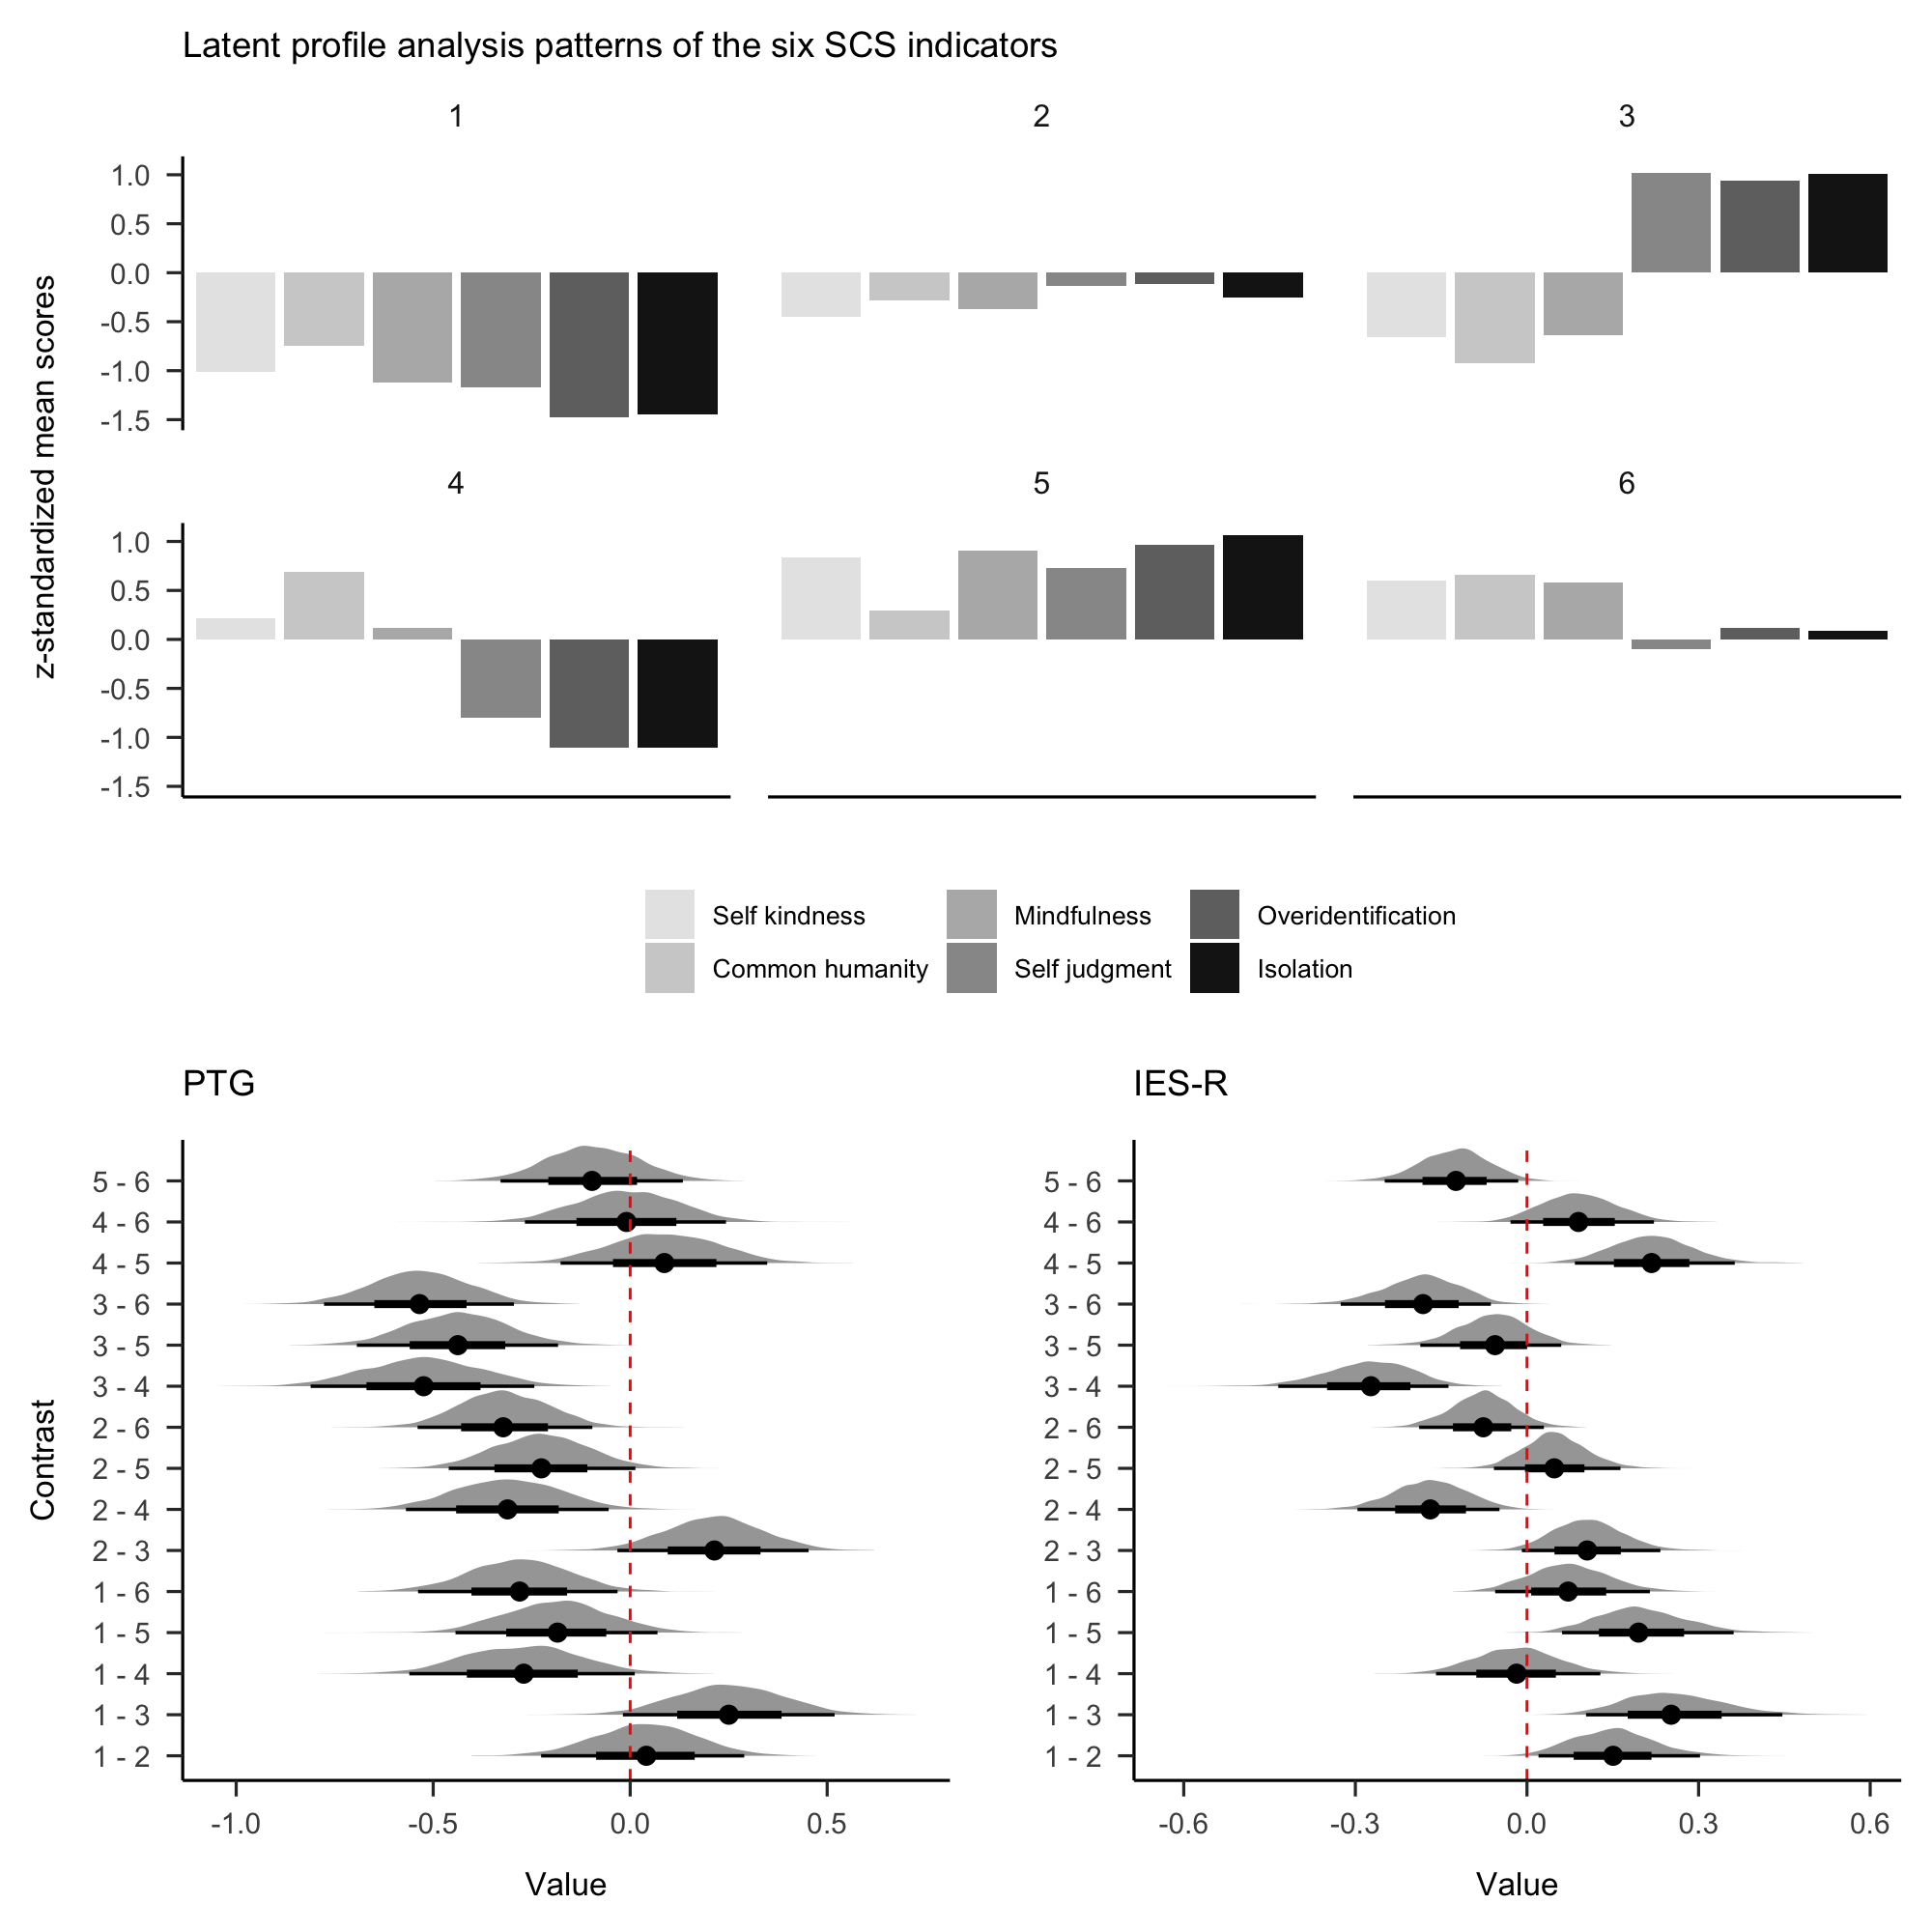
\includegraphics[width=0.94\linewidth]{/Users/corrado/Documents/papers/self_compassion/reports/self_compassion_files/figure-latex/lpa_contrasts} \caption{\textbf{Top.} The first profile (12\% of sample) was labelled \emph{Low CS Low RUS}, because had the lowest relative self-compassion scores on both CS and RUS dimensions; the second profile (21\% of sample), \emph{Medium CS Medium RUS}, was characterized by relatively even scores close to the sample average on both the CS and RUS dimensions; the third profile (15\% of sample), \emph{Low CS High RUS}, was characterized by relatively low levels of the CS dimensions and high levels of the RUS dimension; the fourth profile (13\% of sample), \emph{High CS Low RUS}, was characterized by relatively high levels of the CS dimensions and low levels of the RUS dimension; the fifth profile (19\% of sample), \emph{High CS Low RUS}, was characterized by relatively high levels of both the CS and the RUS dimensions; the sixth profile (19\% of sample), \emph{High CS Medium RUS}, was characterized by relatively high levels of the CS dimension and average levels of the RUS dimension. \textbf{Bottom left.} bla bla. \textbf{Bottom right.} bla bla.}\label{fig:figureLPA}
\end{figure}

\hypertarget{q2-self-compassion-and-level-of-exposure-to-trauma}{%
\subsection{Q2: Self-compassion and level of exposure to trauma}\label{q2-self-compassion-and-level-of-exposure-to-trauma}}

We employed Bayesian regression to examine the associations between the SCS total score and group (rescue workers and a community/student sample not involved in rescue activities), age, gender, and their interactions. We found a group by age interaction, \(\beta\) = -0.19, 95\% CI {[}-0.28, -0.11{]}, Cohen's \emph{d} = 0.21. This interaction indicates that, at the lower age levels, there was no difference between the two groups; conversely, at higher levels of age, rescue workers showed progressively higher levels of the SCS total score as compared to the control group. Bayes R\(^2\) = 0.09. When considering the RUS component as the dependent variable and the same predictors of the previous regression model, we found a similar interaction between group and age as in the previous regression model, \(\beta\) = -0.21, 95\% CI {[}-0.29, -0.12{]}, Cohen's \emph{d} = 0.22. Bayes R\(^2\) = 0.09.
Finally, when considering CS as the dependent variable, we found no reliable effects of group, nor any reliable interaction between group and the other variables. We found an age by gender interaction, \(\beta\) = -0.04, 95\% CI {[}-0.19, -0.02{]}, but the effect size was negligible, Cohen's \emph{d} = 0.11. Bayes R\(^2\) = 0.03.
We interpret these results as indicating that the use of the SCS total score may conceal differences between groups with different levels of exposure to (indirect) trauma.

\hypertarget{q3-the-csrus-components-of-the-scs-and-neuroticism}{%
\subsection{Q3: The CS/RUS components of the SCS and Neuroticism}\label{q3-the-csrus-components-of-the-scs-and-neuroticism}}

To examine the possible separate roles of CS and RUS within a larger nomological network, we compared a number of alternative structural equation models (SEMs). In the context of the concurring effects of coping, perceived social support, and nevroticism, we asked (1) whether the effects of self-compassion on post-traumatic growth and post-traumatic stress symptoms are better accounted for by considering self-compassion as a unitary construct or by distinguishing between CS and RUS; and (2) whether self-compassion is better understood as an exogeneous or as a mediator variable.

\hypertarget{cs-and-rus-as-exogenous-variables}{%
\subsubsection{CS and RUS as exogenous variables}\label{cs-and-rus-as-exogenous-variables}}

\begin{figure}
\centering
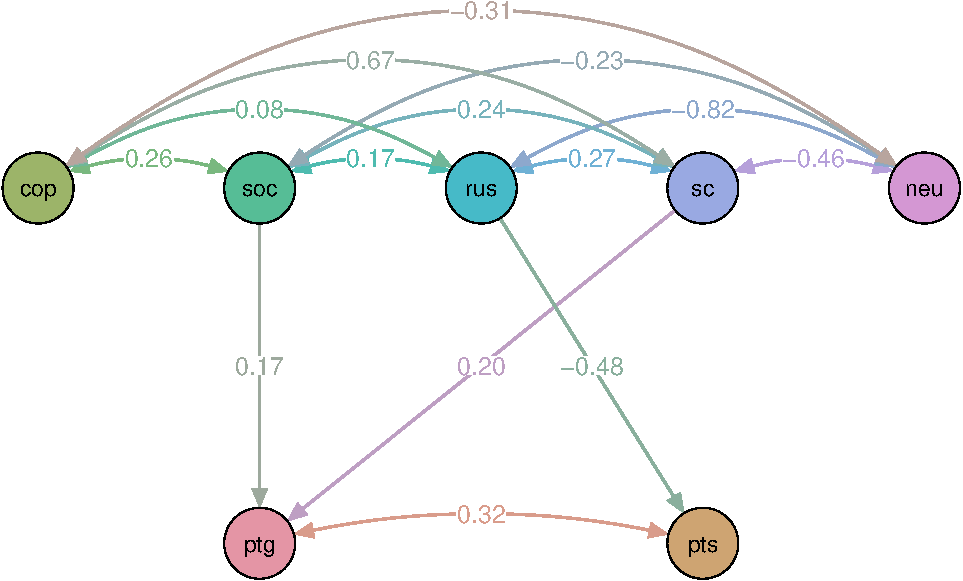
\includegraphics{validity_self_compassion_files/figure-latex/semplot-1.pdf}
\caption{\label{fig:semplot}Direct effects of coping (\texttt{cop}), perceived social support (\texttt{soc}), Reduced Uncompassionate Self-responding (\texttt{rus}), Compassionate Self-responding (\texttt{sc}), neuroticism (\texttt{neu}) on Post-Traumatic Growth (\texttt{ptg}) and Post-Traumatic Stress (\texttt{pts}).}
\end{figure}

Model 3 considers the two separate components of the SCS (RUS and CS), Coping, Social support, and Nevroticism as exogeneous variables, and PTG and PTS as endogeneous variables, taking the sub-scales as indicators of latent factors. The structural component of Model 3 is presented in Figure \ref{fig:semplot} (only the statistical significant path coefficients at the \(\alpha\) = 0.05 level are shown). The model's fit is adequate, \(\chi^2\)(167) = 617.86, \(\chi^2\)/df = 3.70, CFI = 0.95, NFI = 0.93, TLI = 0.93, RMSEA = 0.06, and SRMS = 0.06 (for details, see Supplementary Material). Two model's modifications were considered to tested additional substantive questions. Model 4 removed from Model 3 the direct regression paths from RUS to the endogenous factors. Removing the direct RUS effects decreased the model fit, \(\Delta \chi^2\)(2) = 19.69, \(p =\) 0.00. Model 5 removed from Model 3 the direct regression paths from CS to the endogenous factors. Also removing the direct CS effects decreased the model fit, \(\Delta \chi^2\)(2) = 7.07, \(p =\) 0.03.

\hypertarget{cs-and-rus-as-mediator-variables}{%
\subsubsection{CS and RUS as mediator variables}\label{cs-and-rus-as-mediator-variables}}

\begin{figure}
\centering
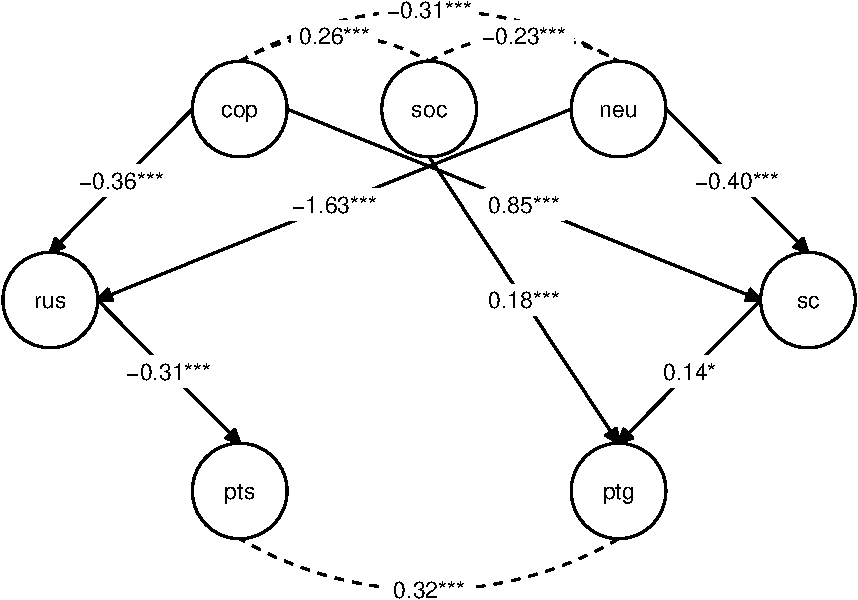
\includegraphics{validity_self_compassion_files/figure-latex/mediation-model-1.pdf}
\caption{\label{fig:mediation-model}Structural component of a SEM model with CS and RUS as mediators between coping, perceived social support, and neuroticism, as exogeneous variables, and Post-Traumatic Growth (\texttt{ptg}) and Post-Traumatic Stress (\texttt{pts}), as endogeneous variables. \texttt{cop} = coping, \texttt{soc} = perceived social support, \texttt{rus} = Reduced Uncompassionate Self-responding, \texttt{sc} = Compassionate Self-responding, \texttt{neu} = neuroticism.}
\end{figure}

Model 6 placed CS and RUS as mediators between Coping, Perceived social support, and Neuroticism (as exogeneous variables), and PTG and PTS (as endogeneous variables). Model-fitting parameters were indicative of good overall
fit: \(\chi^2\)(168) = 618.00, \(\chi^2\)/df = 3.68, CFI = 0.95, NFI = 0.93, TLI = 0.93, RMSEA = 0.06, and SRMS = 0.06. The structural component of Model 6 is presented in Figure \ref{fig:mediation-model} (only the statistical significant path coefficients at the \(\alpha\) = 0.05 level are shown).

We used SEM to answer several substantive questions. Model 7 was identical to Model 6, except that self-compassion was considered as a single latent variable with six indicators. By not distinguishing between the CS and RUS, model fit decreased in comparison to Model 6: \(\Delta \chi^2\)(5) = 640.96, \(p =\) 0.00. In a further modification of Model 6, we considered Neuroticism as a mediator variable rather than an exogenous variable, together with CS and RUS. Compared to Model 6, the model fit decreased: \(\Delta \chi^2\)(2) = 2,010.70, \(p =\) 0.

\begin{table}

\caption{\label{tab:mediation-tab}Indirect and total effects for the three endogeneous variables Coping (coping), Perceived social support (soc. supp.), and Neuroticism (neuro.) on post traumatic stress (PTSS) and post traumatic growth (PTG). S.E. = standard error; `C.I. lower` and `C.I. upper` = lower and upper limits of the 95\% bootstrap confidence interval.}
\centering
\begin{tabular}[t]{lrrrr}
\toprule
Effect & Estimate & S.E. & C.I. lower & C.I. upper\\
\midrule
Ind. eff. Coping -> PTS & 0.10 & 0.06 & -0.03 & 0.22\\
Ind. eff. Coping -> PTG & 0.14 & 0.06 & 0.02 & 0.26\\
Tot. eff. Coping -> PTS & 0.19 & 0.07 & 0.07 & 0.33\\
Tot. eff. Coping -> PTG & 0.24 & 0.06 & 0.13 & 0.35\\
Ind. eff. Soc. supp. -> PTS & -0.01 & 0.02 & -0.06 & 0.04\\
\addlinespace
Ind. eff. Soc. supp. -> PTG & 0.00 & 0.01 & -0.02 & 0.03\\
Tot. eff. Soc. supp. -> PTS & 0.05 & 0.06 & -0.06 & 0.17\\
Tot. eff. Soc. supp. -> PTG & 0.18 & 0.05 & 0.08 & 0.28\\
Ind. eff. Neuro. -> PTS & 0.50 & 0.12 & 0.28 & 0.76\\
Ind. eff. Neuro. -> PTG & 0.03 & 0.10 & -0.18 & 0.23\\
\addlinespace
Tot. eff. Neuro. -> PTS & 0.57 & 0.07 & 0.45 & 0.71\\
Tot. eff. Neuro. -> PTG & 0.15 & 0.05 & 0.05 & 0.25\\
\bottomrule
\end{tabular}
\end{table}

To ask whether CS and RUS are better understood as endogenous variables or as mediators, we compared Models 3 and Model 6 with the Vuong closeness test. Such comparison indicated that Models 3 and 6 were too close too be distinguished, \(p\) = 0.74. However, the confidence intervals for the difference in the models' AIC and BIC statistics showed an advantage for the mediation Model 6: 95\% C.I. of AIC difference = (0.14, 3.60) and 95\% C.I. of BIC difference = (4.73, 8.19). This suggests an advantage for the mediation Model 6 over Model 3.

In order to examine more closely the mediation structure, we computed the bias-corrected bootstrapped confidence interval with 10,000 samples. Such approach does not rely on distribution assumptions and can be used when the assumptions of large sample size and multivariate normality may not hold (Ryu \& Cheong, 2017). If the 95\% confidence intervals do not include zero, this is taken as evidence that the mediation effect is non-zero. We found no evidence of a direct effect of Coping on neither PTG nor on PTSS. Conversely, we found evidence of an indirect effect of Coping on PTG, with a total effect of 0.238, 95\% CI = {[}0.127, 0.355{]}. This suggests a fully mediated effect of Coping on PTG. Instead, no evidence was found of a mediated effect of Coping on PTSS, 95\% CI = {[}-0.026, 0.219{]}. We found no evidence of a direct effect of Perceived social support on PTSS, nor evidence of an indirect effect, 95\% CI = {[}-0.057, 0.037{]}. Instead, we found evidence of a direct effect of perceived social support on PTG, but no evidence of an indirect effect, 95\% CI = {[}-0.023, 0.031{]}; for the total effect, 95\% CI = {[}0.085, 0.282{]}. Finally, we found no evidence of a direct effect of Neuroticism on PTSS, but we found evidence of an indirect effect, 95\% CI = {[}0.283, 0.755{]}, with a total effect of 0.571, 95\% CI = {[}0.451, 0.711{]}. This suggests that the effect of Neuroticism on PTSS is fully mediated. Conversely, we found no evidence of a direct effect of Neuroticism on PTG, nor evidence of an indirect effect of Neuroticism on PTG, with a total effect of 0.032, 95\% CI = {[}-0.184, 0.232{]}.

\hypertarget{discussion}{%
\section{Discussion}\label{discussion}}

Based on the present results, we provide the following responses to the three questions that have motivated the present study. About Question Q1, we found that, in our sample, the best factor structure for the SCS is provided by the six-factor correlated solution, both in ESEM models and in bifactor ESEM models (see Neff et al., 2019). However, we also found that a factor structure which distinguishes between the CS and RUS components of the SCS provides an adequate fit to the data (\emph{e.g.}, Coroiu et al., 2018). We speculate that this result may be due to the specific characteristics of our sample. Rescue workers are constantly confronted with the sufferance of others, a phenomenological condition which is markedly different from the living experience of community participants and undergraduate students who had been often (although not exclusively) employed in previous studies. Exposure to the sufferance of others may encourage loving-kindness (metta), which entails directing a sense of compassion toward oneself and the others, and produces stronger self-care and greater inter-connectedness. Different populations may thus be characterized by different levels of compassionate responding and reduced uncompassionate responding.

Our SEM analyses show that CS offered additional explanatory power to what was offered by RUS; correspondingly, RUS offered additional explanatory power to what was offered by CS. This is an important result which indicates that self-compassion cannot be reduced to the RUS dimension only (\emph{e.g.}, Muris et al., 2019).

The dichotomy between CS and RUS was confirmed when considering the SCS profiles identified by LPA: the CS sub-scales were mainly associated with group differences in PTG, whereas the RUS sub-scales were mainly associated with group differences in IES-R. This suggests that the CS and RUS components of the SCS measure psychological dimensions serving different functional purposes.

When considering the nomological structure that relate self-compassion to other psychological variables, we found that the relations between the examined variables was better described by distinguishing the CS and RUS components of the SCS, rather than by considering self-compassion as a unitary construct. The two components of self-compassion had different effects on PTG and PTS. When CS and RUS were considered as exogenous variables, SC had a direct effect on PTG (but not on PTS), whereas RUS had a direct effect on PTS (but not on PTG) {[}see Fig.~\ref{fig:semplot}{]}. This same pattern was replicated when CS and RUS were considered as mediators. Our data thus suggest that self-compassion is better conceptualized as a bipolar construct.

About Question Q2, we found that the SCS total score and the RUS component increased with age for rescue workers, but for the control group. Instead, no reliable group difference was found in terms of the CS component. These results suggest that, in the present sample, an increased level of (indirect) trauma did not produce compassion fatigue -- \emph{i.e.}, did not produce a decrease of CS which actively enacts kindness and understanding to oneself (self-kindness), recognizes that suffering is a common and normal aspect in life shared by all human beings (common humanity), and achieves a balanced perspective on one's difficulties (mindfulness). Rather, a greater exposure to the sufferance of others promoted an enhancement of the coping strategies with age (\emph{i.e.}, higher levels of RUS). Such ``recalibration of self-compassion'' (\emph{i.e.}, greater defensive attitudes without compromising a proactive positive attitude in relation with the self) is obscured when the CS and RUS components of the SCS are subsumed under a single, overarching dimension (\emph{i.e.}, the SCS total score).

About Question Q3, we found that neuroticism did not overlap with RUS (see, Geiger et al., 2018; Kandler et al., 2017). In fact, we found the opposite result: In a SEM model which included both RUS and neuroticism, these two variables played separate roles. This result is consistent with what found by Neff et al. (2018).

The present study contributes to the growing literature on the self compassion construct and on the SCS as a psychometric operationalization of this same construct. Neff suggests that the use of the six subscales is to be preferred to the use of the global SCS score as it ``provides more precise and nuanced information'' without ``obscuring key difference between the individual components'' (Neff, 2020, p. 1902). Consistently with this proposal, the present study, while providing psychometric support to the ``holistic'' SCS dimension, also adds that the bidimensional conceptualization of self compassion provides a useful summary description of the six subscales.

In this regard, the LPA results are relevant for understanding how the different SCS subscales are configured within individuals. If CS and RUS were unrelated, then we should expect many individuals with high CS and low RUS levels, or with low CS and high RUS levels. Conversely, if CS and RUS dimensions are distinct ``but form a balanced system'' (Neff, 2020, p. 1906), then most individuals should either be high in CS and high in RUS, or low in CS and low in RUS, or moderate in both. As indicated by Figure 1 (top), profiles 1, 2, and 5 are consistent with the second alternative mentioned above (52\% of the sample size), whereas profiles 3, 4, 6 (48\% of the sample) are consistent with the first alternative. This indicates that, in the present sample, the fraction of individuals for whom the configuration of the SCS subscales is consistent with the idea that CS and RUS represent separate dimensions is far from marginal. These results do not replicate those of Phillips (2019; but see also Ullrich-French and Cox, 2020). We speculate that these differences may be due to the fact that self-compassion is expressed in different forms in individuals that are often confronted with the sufferance of others and in community samples or college students. The present considerations, together the previous results concerning the associations between CS and RUS, on the one side, and PTG and PTS, on the other, strengthen the idea that CS and RUS are functionally different components of self compassion.

\hypertarget{limitations-and-future-directions}{%
\subsection{Limitations and future directions}\label{limitations-and-future-directions}}

Limitations include the cross-sectional design, which precludes determination of the development and of the causal role of the risk and protective functions of the self-compassion dimensions. Developmental studies would be important to understand whether the CS and RUS dimensions change over time, and to isolate the factors responsible for such changes.

A strength of the study is the use of a sample of rescue workers. Given the direct personal relevance of the experiences of suffering and failure in rescue workers, in such a sample the study of self-compassion (\emph{i.e.}, of an adaptive response to stress) is facilitated. At the same time, however, the use of such an extreme and specific sample raises the question of the degree to which the present results can generalize to individuals who are engaged to a lesser extent in situations of difficulty or adversity. Therefore, an important extension of this study would be to examine the associations of self-compassion dimensions to adaptive/disadaptive psychological functioning at different levels of context specificity.

Self-compassion can be studied in the context of developmental processes, or as an interactive process in real time. Both when considered as a developmental process or an episodic process, self-compassion is recruited in response to situational demands (environmental or intrapsychic), and is shaped by the individual's resources. From this perspective, the open questions involve the understanding of how particular social contexts, demands, social factors, and individual differences in specific abilities (\emph{e.g.}, cognitive flexibility) shape self-compassion, and whether these factors affect the self-compassion components differently.

Of particular importance would be studying, within clinical settings, the effectiveness of interventions aimed at strengthening self-compassion as a protective factor. Specifically, it would be important to understand of the effectiveness of tailored interventions based on specific patterns of self-compassion dimensions (\emph{i.e.}, deficits in the CS component as distinguished from deficits in the RUS component, or the other way around).

\newpage

\hypertarget{references}{%
\section{References}\label{references}}

\begingroup
\setlength{\parindent}{-0.5in}
\setlength{\leftskip}{0.5in}

\hypertarget{refs}{}
\begin{CSLReferences}{1}{0}
\leavevmode\hypertarget{ref-adams2006compassion}{}%
Adams, R. E., Boscarino, J. A., \& Figley, C. R. (2006). Compassion fatigue and psychological distress among social workers: A validation study. \emph{American Journal of Orthopsychiatry}, \emph{76}(1), 103--108.

\leavevmode\hypertarget{ref-allen2010self}{}%
Allen, A. B., \& Leary, M. R. (2010). Self-compassion, stress, and coping. \emph{Social and Personality Psychology Compass}, \emph{4}(2), 107--118.

\leavevmode\hypertarget{ref-asparouhov2009exploratory}{}%
Asparouhov, T., \& Muthén, B. (2009). Exploratory structural equation modeling. \emph{Structural Equation Modeling: A Multidisciplinary Journal}, \emph{16}(3), 397--438.

\leavevmode\hypertarget{ref-aspy2017mindfulness}{}%
Aspy, D. J., \& Proeve, M. (2017). Mindfulness and loving-kindness meditation: Effects on connectedness to humanity and to the natural world. \emph{Psychological Reports}, \emph{120}(1), 102--117.

\leavevmode\hypertarget{ref-badour2013trauma}{}%
Badour, C. L., \& Feldner, M. T. (2013). Trauma-related reactivity and regulation of emotion: Associations with posttraumatic stress symptoms. \emph{Journal of Behavior Therapy and Experimental Psychiatry}, \emph{44}(1), 69--76.

\leavevmode\hypertarget{ref-bandalos2014relative}{}%
Bandalos, D. L. (2014). Relative performance of categorical diagonally weighted least squares and robust maximum likelihood estimation. \emph{Structural Equation Modeling: A Multidisciplinary Journal}, \emph{21}(1), 102--116.

\leavevmode\hypertarget{ref-barlow2017trauma}{}%
Barlow, M. R., Turow, R. E. G., \& Gerhart, J. (2017). Trauma appraisals, emotion regulation difficulties, and self-compassion predict posttraumatic stress symptoms following childhood abuse. \emph{Child Abuse \& Neglect}, \emph{65}, 37--47.

\leavevmode\hypertarget{ref-beck2016self}{}%
Beck, A. T. (2016). \emph{The self in understanding and treating psychological disorders}. Cambridge University Press.

\leavevmode\hypertarget{ref-berger2012rescuers}{}%
Berger, W., Coutinho, E. S. F., Figueira, I., Marques-Portella, C., Luz, M. P., Neylan, T. C., Marmar, C. R., \& Mendlowicz, M. V. (2012). Rescuers at risk: A systematic review and meta-regression analysis of the worldwide current prevalence and correlates of PTSD in rescue workers. \emph{Social Psychiatry and Psychiatric Epidemiology}, \emph{47}(6), 1001--1011.

\leavevmode\hypertarget{ref-bistricky2017frequency}{}%
Bistricky, S. L., Gallagher, M. W., Roberts, C. M., Ferris, L., Gonzalez, A. J., \& Wetterneck, C. T. (2017). Frequency of interpersonal trauma types, avoidant attachment, self-compassion, and interpersonal competence: A model of persisting posttraumatic symptoms. \emph{Journal of Aggression, Maltreatment \& Trauma}, \emph{26}(6), 608--625.

\leavevmode\hypertarget{ref-caprara2001brand}{}%
Caprara, G. V., Barbaranelli, C., \& Guido, G. (2001). Brand personality: How to make the metaphor fit? \emph{Journal of Economic Psychology}, \emph{22}(3), 377--395.

\leavevmode\hypertarget{ref-carver1989assessing}{}%
Carver, C. S., Scheier, M. F., \& Weintraub, J. K. (1989). Assessing coping strategies: A theoretically based approach. \emph{Journal of Personality and Social Psychology}, \emph{56}(2), 267--283.

\leavevmode\hypertarget{ref-chen2007sensitivity}{}%
Chen, F. F. (2007). Sensitivity of goodness of fit indexes to lack of measurement invariance. \emph{Structural Equation Modeling: A Multidisciplinary Journal}, \emph{14}(3), 464--504.

\leavevmode\hypertarget{ref-cheung2002evaluating}{}%
Cheung, G. W., \& Rensvold, R. B. (2002). Evaluating goodness-of-fit indexes for testing measurement invariance. \emph{Structural Equation Modeling}, \emph{9}(2), 233--255.

\leavevmode\hypertarget{ref-chishima2018influence}{}%
Chishima, Y., Mizuno, M., Sugawara, D., \& Miyagawa, Y. (2018). The influence of self-compassion on cognitive appraisals and coping with stressful events. \emph{Mindfulness}, \emph{9}(6), 1907--1915.

\leavevmode\hypertarget{ref-coroiu2018structural}{}%
Coroiu, A., Kwakkenbos, L., Moran, C., Thombs, B., Albani, C., Bourkas, S., Zenger, M., Brahler, E., \& Körner, A. (2018). Structural validation of the self-compassion scale with a german general population sample. \emph{PloS One}, \emph{13}(2), e0190771.

\leavevmode\hypertarget{ref-costa1992normal}{}%
Costa, P. T., \& McCrae, R. R. (1992). Normal personality assessment in clinical practice: The NEO personality inventory. \emph{Psychological Assessment}, \emph{4}(1), 5--13.

\leavevmode\hypertarget{ref-craparo2013impact}{}%
Craparo, G., Faraci, P., Rotondo, G., \& Gori, A. (2013). The impact of event scale--revised: Psychometric properties of the italian version in a sample of flood victims. \emph{Neuropsychiatric Disease and Treatment}, \emph{9}, 1427--1432.

\leavevmode\hypertarget{ref-creamer2003psychometric}{}%
Creamer, M., Bell, R., \& Failla, S. (2003). Psychometric properties of the impact of event scale---revised. \emph{Behaviour Research and Therapy}, \emph{41}(12), 1489--1496.

\leavevmode\hypertarget{ref-fabio2012emotional}{}%
Fabio, A. D., \& Kenny, M. E. (2012). Emotional intelligence and perceived social support among italian high school students. \emph{Journal of Career Development}, \emph{39}(5), 461--475.

\leavevmode\hypertarget{ref-geiger2018self}{}%
Geiger, M., Pfattheicher, S., Hartung, J., Weiss, S., Schindler, S., Wilhelm, O., \& Kandler, C. (2018). Self--compassion as a facet of neuroticism? A reply to the comments of {Neff, T{ó}Th--Kir{á}Ly, and Colosimo (2018)}. \emph{European Journal of Personality}, \emph{32}(4), 393--404.

\leavevmode\hypertarget{ref-gu2020development}{}%
Gu, J., Baer, R., Cavanagh, K., Kuyken, W., \& Strauss, C. (2020). Development and psychometric properties of the sussex-oxford compassion scales (SOCS). \emph{Assessment}, \emph{27}(1), 3--20.

\leavevmode\hypertarget{ref-janoff1989assumptive}{}%
Janoff-Bulman, R. (1989). Assumptive worlds and the stress of traumatic events: Applications of the schema construct. \emph{Social Cognition}, \emph{7}(2), 113--136.

\leavevmode\hypertarget{ref-kandler2017old}{}%
Kandler, C., Pfattheicher, S., Geiger, M., Hartung, J., Weiss, S., \& Schindler, S. (2017). Old wine in new bottles? The case of self--compassion and neuroticism. \emph{European Journal of Personality}, \emph{31}(2), 160--169.

\leavevmode\hypertarget{ref-keene2016childhood}{}%
Keene, A. C., \& Epps, J. (2016). Childhood physical abuse and aggression: Shame and narcissistic vulnerability. \emph{Child Abuse \& Neglect}, \emph{51}, 276--283.

\leavevmode\hypertarget{ref-kirby2017meta}{}%
Kirby, J. N., Tellegen, C. L., \& Steindl, S. R. (2017). A meta-analysis of compassion-based interventions: Current state of knowledge and future directions. \emph{Behavior Therapy}, \emph{48}(6), 778--792.

\leavevmode\hypertarget{ref-little2013longitudinal}{}%
Little, T. D. (2013). \emph{Longitudinal structural equation modeling}. Guilford press.

\leavevmode\hypertarget{ref-macbeth2012exploring}{}%
MacBeth, A., \& Gumley, A. (2012). Exploring compassion: A meta-analysis of the association between self-compassion and psychopathology. \emph{Clinical Psychology Review}, \emph{32}(6), 545--552.

\leavevmode\hypertarget{ref-montero2018self}{}%
Montero-Marin, J., Kuyken, W., Crane, C., Gu, J., Baer, R., Al-Awamleh, A. A., Akutsu, S., Araya-Véliz, C., Ghorbani, N., Chen, Z. J., \& others. (2018). Self-compassion and cultural values: A cross-cultural study of self-compassion using a multitrait-multimethod (MTMM) analytical procedure. \emph{Frontiers in Psychology}, \emph{9}, 2638.

\leavevmode\hypertarget{ref-muris2016protective}{}%
Muris, P. (2016). A protective factor against mental health problems in youths? A critical note on the assessment of self-compassion. \emph{Journal of Child and Family Studies}, \emph{25}(5), 1461--1465.

\leavevmode\hypertarget{ref-muris2018good}{}%
Muris, P., Broek, M. van den, Otgaar, H., Oudenhoven, I., \& Lennartz, J. (2018). Good and bad sides of self-compassion: A face validity check of the self-compassion scale and an investigation of its relations to coping and emotional symptoms in non-clinical adolescents. \emph{Journal of Child and Family Studies}, \emph{27}(8), 2411--2421.

\leavevmode\hypertarget{ref-muris2020process}{}%
Muris, P., \& Otgaar, H. (2020). The process of science: A critical evaluation of more than 15 years of research on self-compassion with the self-compassion scale. \emph{Mindfulness}, \emph{11}(6), 1469--1482.

\leavevmode\hypertarget{ref-muris2021non}{}%
Muris, P., Otgaar, H., López, A., Kurtic, I., \& Laar, I. van de. (2021). The (non) protective role of self-compassion in internalizing symptoms: Two empirical studies in adolescents demonstrating unwanted effects of using the self-compassion scale total score. \emph{Mindfulness}, \emph{12}(1), 240--252.

\leavevmode\hypertarget{ref-muris2016protection}{}%
Muris, P., Otgaar, H., \& Petrocchi, N. (2016). Protection as the mirror image of psychopathology: Further critical notes on the self-compassion scale. \emph{Mindfulness}, \emph{7}(3), 787--790.

\leavevmode\hypertarget{ref-muris2019stripping}{}%
Muris, P., Otgaar, H., \& Pfattheicher, S. (2019). Stripping the forest from the rotten trees: Compassionate self-responding is a way of coping, but reduced uncompassionate self-responding mainly reflects psychopathology. \emph{Mindfulness}, \emph{10}(1), 196--199.

\leavevmode\hypertarget{ref-muris2017protection}{}%
Muris, P., \& Petrocchi, N. (2017). Protection or vulnerability? A meta-analysis of the relations between the positive and negative components of self-compassion and psychopathology. \emph{Clinical Psychology \& Psychotherapy}, \emph{24}(2), 373--383.

\leavevmode\hypertarget{ref-murray2003neo}{}%
Murray, G., Rawlings, D., Allen, N. B., \& Trinder, J. (2003). NEO five-factor inventory scores: Psychometric properties in a community sample. \emph{Measurement and Evaluation in Counseling and Development}, \emph{36}(3), 140--149.

\leavevmode\hypertarget{ref-muthen2017mplus}{}%
Muthén, B., \& Muthén, B. O. (2017). Mplus. \emph{Statistical Analysis with Latent Variables. User's Guide}, \emph{8}.

\leavevmode\hypertarget{ref-muthen2015estimator}{}%
Muthén, B. O., Muthén, L., \& Asparouhov, T. (2015). Estimator choices with categorical outcomes. \emph{MPLUS Technical Appendix}, \emph{8}.

\leavevmode\hypertarget{ref-neff2003self}{}%
Neff, K. D. (2003a). Self-compassion: An alternative conceptualization of a healthy attitude toward oneself. \emph{Self and Identity}, \emph{2}(2), 85--101.

\leavevmode\hypertarget{ref-neff2003development}{}%
Neff, K. D. (2003b). The development and validation of a scale to measure self-compassion. \emph{Self and Identity}, \emph{2}(3), 223--250.

\leavevmode\hypertarget{ref-neff2020commentary}{}%
Neff, K. D. (2020). Commentary on muris and otgaar (2020): Let the empirical evidence speak on the self-compassion scale. \emph{Mindfulness}, \emph{11}, 1900--1909.

\leavevmode\hypertarget{ref-neff2018self}{}%
Neff, K. D., Tóth--Király, I., Colosimo, K., \& Kandler, C. (2018). Self--compassion is best measured as a global construct and is overlapping with but distinct from neuroticism: A response to pfattheicher, geiger, hartung, weiss, and schindler (2017). \emph{European Journal of Personality}, \emph{32}(4), 371--392.

\leavevmode\hypertarget{ref-neff2019examining}{}%
Neff, K. D., Tóth-Király, I., Yarnell, L. M., Arimitsu, K., Castilho, P., Ghorbani, N., Guo, H. X., Hirsch, J. K., Hupfeld, J., Hutz, C. S., \& others. (2019). Examining the factor structure of the self-compassion scale in 20 diverse samples: Support for use of a total score and six subscale scores. \emph{Psychological Assessment}, \emph{31}(1), 27--45.

\leavevmode\hypertarget{ref-nolen2008rethinking}{}%
Nolen-Hoeksema, S., Wisco, B. E., \& Lyubomirsky, S. (2008). Rethinking rumination. \emph{Perspectives on Psychological Science}, \emph{3}(5), 400--424.

\leavevmode\hypertarget{ref-palgi2009effect}{}%
Palgi, Y., Ben-Ezra, M., Langer, S., \& Essar, N. (2009). The effect of prolonged exposure to war stress on the comorbidity of PTSD and depression among hospital personnel. \emph{Psychiatry Research}, \emph{168}(3), 262--264.

\leavevmode\hypertarget{ref-phillips2019self}{}%
Phillips, W. J. (2019). Self-compassion mindsets: The components of the self-compassion scale operate as a balanced system within individuals. \emph{Current Psychology}, 1--14.

\leavevmode\hypertarget{ref-prati2014italian}{}%
Prati, G., \& Pietrantoni, L. (2014). Italian adaptation and confirmatory factor analysis of the full and the short form of the posttraumatic growth inventory. \emph{Journal of Loss and Trauma}, \emph{19}(1), 12--22.

\leavevmode\hypertarget{ref-prezza2002perceived}{}%
Prezza, M., \& Giuseppina Pacilli, M. (2002). Perceived social support from significant others, family and friends and several socio-demographic characteristics. \emph{Journal of Community \& Applied Social Psychology}, \emph{12}(6), 422--429.

\leavevmode\hypertarget{ref-ryu2017comparing}{}%
Ryu, E., \& Cheong, J. (2017). Comparing indirect effects in different groups in single-group and multi-group structural equation models. \emph{Frontiers in Psychology}, \emph{8}, 747.

\leavevmode\hypertarget{ref-seligowski2015relations}{}%
Seligowski, A. V., Miron, L. R., \& Orcutt, H. K. (2015). Relations among self-compassion, PTSD symptoms, and psychological health in a trauma-exposed sample. \emph{Mindfulness}, \emph{6}(5), 1033--1041.

\leavevmode\hypertarget{ref-seppala2017oxford}{}%
Seppälä, E. M., Simon-Thomas, E., Brown, S. L., Worline, M. C., Cameron, C. D., \& Doty, J. R. (2017). \emph{The oxford handbook of compassion science}. Oxford University Press.

\leavevmode\hypertarget{ref-sica2008coping}{}%
Sica, C., Magni, C., Ghisi, M., Altoè, G., Sighinolfi, C., Chiri, L. R., \& Franceschini, S. (2008). Coping orientation to problems experienced-nuova versione italiana (COPE-NVI): Uno strumento per la misura degli stili di coping. \emph{Psicoterapia Cognitiva e Comportamentale}, \emph{14}(1), 27.

\leavevmode\hypertarget{ref-sica1997coping}{}%
Sica, C., Novara, C., Dorz, S., \& Sanavio, E. (1997). Coping strategies: Evidence for cross-cultural differences? A preliminary study with the italian version of coping orientations to problems experienced (COPE). \emph{Personality and Individual Differences}, \emph{23}(6), 1025--1029.

\leavevmode\hypertarget{ref-siefert2020development}{}%
Siefert, C. J., Sexton, J., Meehan, K., Nelson, S., Haggerty, G., Dauphin, B., \& Huprich, S. (2020). Development of a short form for the DSM--5 levels of personality functioning questionnaire. \emph{Journal of Personality Assessment}, \emph{102}(4), 516--526.

\leavevmode\hypertarget{ref-sodeke2013compassion}{}%
Sodeke-Gregson, E. A., Holttum, S., \& Billings, J. (2013). Compassion satisfaction, burnout, and secondary traumatic stress in UK therapists who work with adult trauma clients. \emph{European Journal of Psychotraumatology}, \emph{4}(1), 21869.

\leavevmode\hypertarget{ref-strauss2016compassion}{}%
Strauss, C., Taylor, B. L., Gu, J., Kuyken, W., Baer, R., Jones, F., \& Cavanagh, K. (2016). What is compassion and how can we measure it? A review of definitions and measures. \emph{Clinical Psychology Review}, \emph{47}, 15--27.

\leavevmode\hypertarget{ref-tedeschi1996posttraumatic}{}%
Tedeschi, R. G., \& Calhoun, L. G. (1996). The posttraumatic growth inventory: Measuring the positive legacy of trauma. \emph{Journal of Traumatic Stress}, \emph{9}(3), 455--471.

\leavevmode\hypertarget{ref-tedeschi2004posttraumatic}{}%
Tedeschi, R. G., \& Calhoun, L. G. (2004). " posttraumatic growth: Conceptual foundations and empirical evidence". \emph{Psychological Inquiry}, \emph{15}(1), 1--18.

\leavevmode\hypertarget{ref-ullrich2020use}{}%
Ullrich-French, S., \& Cox, A. E. (2020). The use of latent profiles to explore the multi-dimensionality of self-compassion. \emph{Mindfulness}, \emph{11}, 1483--1499.

\leavevmode\hypertarget{ref-veneziani2017self}{}%
Veneziani, C. A., Fuochi, G., \& Voci, A. (2017). Self-compassion as a healthy attitude toward the self: Factorial and construct validity in an italian sample. \emph{Personality and Individual Differences}, \emph{119}, 60--68.

\leavevmode\hypertarget{ref-wadsworth2018examining}{}%
Wadsworth, L. P., Forgeard, M., Hsu, K. J., Kertz, S., Treadway, M., \& Björgvinsson, T. (2018). Examining the role of repetitive negative thinking in relations between positive and negative aspects of self-compassion and symptom improvement during intensive treatment. \emph{Cognitive Therapy and Research}, \emph{42}(3), 236--249.

\leavevmode\hypertarget{ref-weiss2007impact}{}%
Weiss, D. S. (2007). The impact of event scale: revised. In \emph{Cross-cultural assessment of psychological trauma and PTSD} (pp. 219--238). Springer.

\leavevmode\hypertarget{ref-west2012model}{}%
West, S. G., Taylor, A. B., Wu, W., \& others. (2012). Model fit and model selection in structural equation modeling. \emph{Handbook of Structural Equation Modeling}, \emph{1}, 209--231.

\leavevmode\hypertarget{ref-wilson2019effectiveness}{}%
Wilson, A. C., Mackintosh, K., Power, K., \& Chan, S. W. (2019). Effectiveness of self-compassion related therapies: A systematic review and meta-analysis. \emph{Mindfulness}, \emph{10}(6), 979--995.

\leavevmode\hypertarget{ref-winders2020self}{}%
Winders, S.-J., Murphy, O., Looney, K., \& O'Reilly, G. (2020). Self-compassion, trauma, and posttraumatic stress disorder: A systematic review. \emph{Clinical Psychology \& Psychotherapy}, \emph{27}(3), 300--329.

\leavevmode\hypertarget{ref-witteveen2007psychological}{}%
Witteveen, A. B., Bramsen, I., Twisk, J. W., Huizink, A. C., Slottje, P., Smid, T., \& Van Der Ploeg, H. M. (2007). Psychological distress of rescue workers eight and one-half years after professional involvement in the amsterdam air disaster. \emph{The Journal of Nervous and Mental Disease}, \emph{195}(1), 31--40.

\leavevmode\hypertarget{ref-wong2017self}{}%
Wong, C. C. Y., \& Yeung, N. C. (2017). Self-compassion and posttraumatic growth: Cognitive processes as mediators. \emph{Mindfulness}, \emph{8}(4), 1078--1087.

\leavevmode\hypertarget{ref-zimet1988multidimensional}{}%
Zimet, G. D., Dahlem, N. W., Zimet, S. G., \& Farley, G. K. (1988). The multidimensional scale of perceived social support. \emph{Journal of Personality Assessment}, \emph{52}(1), 30--41.

\leavevmode\hypertarget{ref-zimet1990psychometric}{}%
Zimet, G. D., Powell, S. S., Farley, G. K., Werkman, S., \& Berkoff, K. A. (1990). Psychometric characteristics of the multidimensional scale of perceived social support. \emph{Journal of Personality Assessment}, \emph{55}(3-4), 610--617.

\end{CSLReferences}

\newpage

\renewcommand{\appendixname}{Supplementary Information}
\setcounter{page}{1}


\clearpage
\makeatletter
\efloat@restorefloats
\makeatother


\begin{appendix}
\hypertarget{sample-characteristics}{%
\section{Sample characteristics}\label{sample-characteristics}}

Concerning the relation between personality traits and the SCS total
score, we found that the SCS total score was negatively associated with
neuroticism, \(b\) = -0.59, \(SE\) = 0.03, Bayesian 95\% CI {[}-0.65,
-0.53{]} (Neff et al., 2007), and positively associated with
extroversion, \(b\) = 0.10, \(SE\) = 0.03, Bayesian 95\% CI {[}0.03,
0.17{]}, and with agreeableness, \(b\) = 0.07, \(SE\) = 0.03, Bayesian
95\% CI {[}0.01, 0.12{]}. We found no evidence of an association with
level of education, years of experience as rescue worker, time gap since
the last training, and rate of rescue worker activity.

We also found that PTG was positively associated with neuroticism, \(b\)
= 0.19, \(SE\) = 0.05, Bayesian 95\% CI {[}0.10, 0.28{]}, extroversion,
\(b\) = 0.24, \(SE\) = 0.05, Bayesian 95\% CI {[}0.14, 0.33{]},
conscientiousness, \(b\) = 0.10, \(SE\) = 0.04, Bayesian 95\% CI
{[}0.01, 0.18{]}, age, \(b\) = 0.15, \(SE\) = 0.04, Bayesian 95\% CI
{[}0.06, 0.24{]} (see Garnefski et al., 2008), and rate of rescue-worker
activity, \(b\) = 0.08, \(SE\) = 0.04, Bayesian 95\% CI {[}0.00,
0.16{]}; moreover, males showed lower levels of PTG than females, \(b\)
= -0.20, \(SE\) = 0.08, Bayesian 95\% CI {[}-0.36, -0.04{]}.

IES-R scores were positively associated with neuroticism, \(b\) = 0.18,
\(SE\) = 0.04, Bayesian 95\% CI {[}0.11, 0.25{]} (Inoue et al., 2006),
and educational level, \(b\) = -0.06, \(SE\) = 0.02, Bayesian 95\% CI
{[}-0.10, -0.01{]} (Wu et al., 2005), but negatively associated with
age, \(b\) = -0.05, \(SE\) = 0.03, Bayesian 95\% CI {[}-0.10, -0.00{]}.

\newpage

\hypertarget{scs-factor-structure}{%
\section{SCS factor structure}\label{scs-factor-structure}}

We compared the fit of all models discussed by Neff et al. (2019). We
started with the unidimensional CFA model, which clearly proved to be
inadequate, CFI = 0.61, TLI = 0.58, RMSEA = 0.18 {[}90\% CI
0.18-0.19{]}, SRMR = 0.16, \(\omega_t\) = 0.44. We then considered all
the factor structures that had been discussed by Neff et al. (2019). The
list of the examined models, together with their fit indexes, is provide
below:

\begin{itemize}
\item
a two-factor CFA for the positive and the negative components of SC,
CFI = 0.83, TLI = 0.82, RMSEA = 0.12 {[}90\% CI 0.12-0.12{]}, SRMR =
0.10, \(\omega_t\) = 0.96;
\item
a two-factor ESEM, CFI = 0.85, TLI = 0.82, RMSEA = 0.12 {[}90\% CI
0.12-0.12{]}, SRMR = 0.06, \(\omega_t\) = 0.96;
\item
a six-factor CFA, CFI = 0.90, TLI = 0.88, RMSEA = 0.10 {[}90\% CI
0.09-0.10{]}, SRMR = 0.07, \(\omega_t\) = 0.97;
\item
a six-factor ESEM, CFI = 0.98, TLI = 0.96, RMSEA = 0.05 {[}90\% CI
0.05-0.06{]}, SRMR = 0.02, \(\omega_t\) = 0.98;
\item
a bifactor-CFA (1 G- and 6 S-factors), CFI = 0.76, TLI = 0.71, RMSEA =
0.15 {[}90\% CI 0.15-0.16{]}, SRMR = 0.12, \(\omega_t\) = 0.97;
\item
a bifactor-ESEM (1 G- and 6 S-factors), CFI = 0.98, TLI = 0.96, RMSEA
= 0.05 {[}90\% CI 0.05-0.06{]}, SRMR = 0.02, \(\omega_t\) = 0.99;
\item
a two-bifactor (two-tier) CFA model (2 G- and 6 S-factors), CFI =
0.90, TLI = 0.88, RMSEA = 0.10 {[}90\% CI 0.10-0.10{]}, SRMR = 0.08,
\(\omega_t\) = 0.99;
\item
a two-bifactor (two-tier) ESEM model (2 G- and 6 S-factors), CFI =
0.99, TLI = 0.98, RMSEA = 0.04 {[}90\% CI 0.04-0.05{]}, SRMR = 0.01,
\(\omega_t\) = 0.99.
\end{itemize}

For the two-factor CFA for the CS and RUS of SC, the correlation between
the factors was -0.28. For the two-factor ESEM, the correlation between
the factors was -0.21. For the 6-factor CFA, the correlations between
factors ranged between -0.44 and 0.95. For the 6-factor ESEM, the
correlations between factors ranged between -0.36 and 0.58. For the
two-bifactor (two-tier) CFA model (2 G- and 6 S-factors), the
correlation between the CS and RUS factors is -0.34. For the
two-bifactor (two-tier) ESEM model (2 G- and 6 S-factors), the
correlation between the CS and RUS factors is -0.55.

In our sample, the two-bifactor (two-tier) ESEM model, which included 6
uncorrelated factors (self-kindness, reduced self-judgment, common
humanity, reduced isolation, mindfulness, and reduced
over-identification) and two correlated CS (loading on the
self-kindness, common humanity, and mindfulness items) and RUS (loading
on the reduced self-judgment, reduced isolation, and reduced
over-identification items) factors showed a marginally better fit than
the one bifactor-ESEM (1 G- and 6 S-factors) model. What is crucial is
that, among the considered models, those that provide the best fits to
the data include distinct factors corresponding to the six dimensions of
the SCS (self-kindness, reduced self-judgment, common humanity, reduced
isolation, mindfulness, and reduced over-identification).

\newpage

\hypertarget{a-two-factor-correlated-model-with-two-unitary-factors-representing-cs-and-rus}{%
\section{A two-factor correlated model with two unitary factors
representing CS and
RUS}\label{a-two-factor-correlated-model-with-two-unitary-factors-representing-cs-and-rus}}

\hypertarget{mplus-syntax}{%
\subsection{Mplus syntax}\label{mplus-syntax}}

\begin{verbatim}
TITLE: 2 factor ESEM.
DATA:
FILE IS selfcompassionitems.dat;
VARIABLE:
NAMES ARE scsj1 scoi2 scch3 scis4 scsk5 scoi6 scch7 scsj8 
scmi9 scch10 scsj11 scsk12 scis13 scmi14 scch15 
scsj16 scmi17 scis18 scsk19 scoi20 scsj21 scmi22 
scsk23 scoi24 scis25 scsk26; 
MISSING ARE ALL(-9);
USEVARIABLES ARE scsj1 scoi2 scch3 scis4 scsk5 scoi6 scch7 scsj8 
scmi9 scch10 scsj11 scsk12 scis13 scmi14 scch15 
scsj16 scmi17 scis18 scsk19 scoi20 scsj21 scmi22 
scsk23 scoi24 scis25 scsk26; 
CATEGORICAL ARE all;
ANALYSIS:
! Requesting the weighted least squares mean- and variance-adjusted estimator
ESTIMATOR = WLSMV;
ROTATION = target;
MODEL:
pos BY scsk5 scsk12 scsk19 scsk23 scsk26 scsj1~0 scsj8~0 scsj11~0 
scsj16~0 scsj21~0 scch3 scch7 scch10 scch15 scis4~0 scis13~0 
scis18~0 scis25~0 scmi9 scmi14 scmi17 scmi22 scoi2~0 scoi6~0 
scoi20~0 scoi24~0 (*1);
neg BY scsk5~0 scsk12~0 scsk19~0 scsk23~0 scsk26~0 scsj1 scsj8 scsj11 
scsj16 scsj21 scch3~0 scch7~0 scch10~0 scch15~0 scis4 scis13 
scis18 scis25 scmi9~0 scmi14~0 scmi17~0 scmi22~0 scoi2 scoi6 
scoi20 scoi24 (*1);
! Requesting standardized parameter estimates
OUTPUT: stdyx;
\end{verbatim}

\newpage

\hypertarget{standardized-factor-loadings}{%
\subsubsection{Standardized Factor
Loadings}\label{standardized-factor-loadings}}

\captionsetup[table]{labelformat=empty,skip=1pt}
\begin{longtable}{crr}
\toprule
Items & CS & RUS \\ 
\midrule
\multicolumn{1}{l}{Self-kindness} \\ 
\midrule
SCSK05 & 0.69 & 0.12 \\ 
SCSK12 & 0.76 & -0.04 \\ 
SCSK19 & 0.76 & -0.08 \\ 
SCSK23 & 0.60 & -0.27 \\ 
SCSK26 & 0.66 & -0.11 \\ 
\midrule
\multicolumn{1}{l}{Mindfulness} \\ 
\midrule
SCMI09 & 0.52 & 0.06 \\ 
SCMI14 & 0.56 & -0.19 \\ 
SCMI17 & 0.63 & -0.23 \\ 
SCMI22 & 0.66 & -0.08 \\ 
\midrule
\multicolumn{1}{l}{Common Humanity} \\ 
\midrule
SCCH03 & 0.46 & 0.23 \\ 
SCCH07 & 0.57 & 0.40 \\ 
SCCH10 & 0.62 & 0.30 \\ 
SCCH15 & 0.69 & 0.00 \\ 
\midrule
\multicolumn{1}{l}{Self-judgment} \\ 
\midrule
SCSJ01 & 0.07 & 0.55 \\ 
SCSJ08 & 0.02 & 0.77 \\ 
SCSJ11 & 0.03 & 0.74 \\ 
SCSJ16 & -0.01 & 0.74 \\ 
SCSJ21 & 0.03 & 0.60 \\ 
\midrule
\multicolumn{1}{l}{Isolation} \\ 
\midrule
SCIS04 & -0.08 & 0.82 \\ 
SCIS13 & -0.04 & 0.78 \\ 
SCIS18 & 0.02 & 0.82 \\ 
SCIS25 & -0.05 & 0.78 \\ 
\midrule
\multicolumn{1}{l}{Over-identification} \\ 
\midrule
SCOI02 & -0.07 & 0.81 \\ 
SCOI06 & -0.04 & 0.81 \\ 
SCOI20 & 0.04 & 0.67 \\ 
SCOI24 & -0.03 & 0.68 \\ 
\bottomrule
\end{longtable}



\newpage

\hypertarget{a-two-factor-correlated-model-with-two-unitary-factors-representing-cs-and-rus-1}{%
\section{A two-factor correlated model with two unitary factors
representing CS and
RUS}\label{a-two-factor-correlated-model-with-two-unitary-factors-representing-cs-and-rus-1}}

\hypertarget{mplus-syntax-r-factor-extraction}{%
\subsection{Mplus syntax -- R factor
extraction}\label{mplus-syntax-r-factor-extraction}}

\begin{verbatim}
TITLE: 2 factor ESEM v2.
DATA:
FILE IS selfcompassionitems.dat;
VARIABLE:
NAMES ARE scsj1 scoi2 scch3 scis4 scsk5 scoi6 scch7 scsj8 
scmi9 scch10 scsj11 scsk12 scis13 scmi14 scch15 
scsj16 scmi17 scis18 scsk19 scoi20 scsj21 scmi22 
scsk23 scoi24 scis25 scsk26; 
MISSING ARE ALL(-9);
USEVARIABLES ARE scsj1 scoi2 scch3 scis4 scsk5 scoi6 scch7 scsj8 
scmi9 scch10 scsj11 scsk12 scis13 scmi14 scch15 
scsj16 scmi17 scis18 scsk19 scoi20 scsj21 scmi22 
scsk23 scoi24 scis25 scsk26; 
CATEGORICAL ARE all;
ANALYSIS: 
ESTIMATOR = WLSMV; 
ROTATION = oblimin; 
MODEL:
pos BY scsj1@.06 scoi2@-.05 scch3@.41 scis4@-.070 scsk5@.65 scoi6@-.03 
scch7@0.49 scsj8@.01 scmi9@0.46 scch10@0.55 scsj11@.02 scsk12@.69 
scis13@-.04 scmi14@0.47 scch15@0.66 scsj16@-0.01 scmi17@0.58 
scis18@0.03 scsk19@0.70 scoi20@0.07 scsj21@0.02 scmi22@0.65 
scsk23@0.56 scoi24@-0.01 scis25@-0.04 scsk26@0.64;
neg BY scsj1@.49 scoi2@.78 scch3@.22 scis4@.78 scsk5@.13 scoi6@.79 
scch7@.33 scsj8@.70 scmi9@.07 scch10@.24 scsj11@.68 scsk12@-.03 
scis13@.71 scmi14@-.17 scch15@.02 scsj16@.69 scmi17@-.2 
scis18@.77 scsk19@-.06 scoi20@.64 scsj21@.56 scmi22@-.05 
scsk23@-.22 scoi24@0.62 scis25@.75 scsk26@-.06;
pos@1;
neg@1;
OUTPUT: stdyx;
\end{verbatim}

\newpage

\hypertarget{standardized-factor-loadings-1}{%
\subsubsection{Standardized Factor
Loadings}\label{standardized-factor-loadings-1}}

\captionsetup[table]{labelformat=empty,skip=1pt}
\begin{longtable}{crr}
\toprule
Items & CS & RUS \\ 
\midrule
\multicolumn{1}{l}{Self-kindness} \\ 
\midrule
SCSK05 & 0.65 & 0.13 \\ 
SCSK12 & 0.69 & -0.03 \\ 
SCSK19 & 0.70 & -0.06 \\ 
SCSK23 & 0.56 & -0.22 \\ 
SCSK26 & 0.64 & -0.06 \\ 
\midrule
\multicolumn{1}{l}{Mindfulness} \\ 
\midrule
SCMI09 & 0.46 & 0.07 \\ 
SCMI14 & 0.47 & -0.17 \\ 
SCMI17 & 0.58 & -0.20 \\ 
SCMI22 & 0.65 & -0.05 \\ 
\midrule
\multicolumn{1}{l}{Common Humanity} \\ 
\midrule
SCCH03 & 0.41 & 0.22 \\ 
SCCH07 & 0.49 & 0.33 \\ 
SCCH10 & 0.55 & 0.24 \\ 
SCCH15 & 0.66 & 0.02 \\ 
\midrule
\multicolumn{1}{l}{Self-judgment} \\ 
\midrule
SCSJ01 & 0.06 & 0.49 \\ 
SCSJ08 & 0.01 & 0.70 \\ 
SCSJ11 & 0.02 & 0.68 \\ 
SCSJ16 & -0.01 & 0.69 \\ 
SCSJ21 & 0.02 & 0.56 \\ 
\midrule
\multicolumn{1}{l}{Isolation} \\ 
\midrule
SCIS04 & -0.07 & 0.78 \\ 
SCIS13 & -0.04 & 0.71 \\ 
SCIS18 & 0.03 & 0.77 \\ 
SCIS25 & -0.04 & 0.75 \\ 
\midrule
\multicolumn{1}{l}{Over-identification} \\ 
\midrule
SCOI02 & -0.05 & 0.78 \\ 
SCOI06 & -0.03 & 0.79 \\ 
SCOI20 & 0.07 & 0.64 \\ 
SCOI24 & -0.01 & 0.62 \\ 
\bottomrule
\end{longtable}



\newpage

\hypertarget{a-two-correlated-factors-bifactor-model}{%
\section{A two-correlated factors bifactor
model}\label{a-two-correlated-factors-bifactor-model}}

\hypertarget{mplus-syntax-1}{%
\subsection{Mplus syntax}\label{mplus-syntax-1}}

\begin{verbatim}
TITLE: bifactor 2-correlated-factors ESEM.
DATA:
FILE IS selfcompassionitems.dat;
VARIABLE:
NAMES ARE scsj1 scoi2 scch3 scis4 scsk5 scoi6 scch7 scsj8
scmi9 scch10 scsj11 scsk12 scis13 scmi14 scch15
scsj16 scmi17 scis18 scsk19 scoi20 scsj21 scmi22
scsk23 scoi24 scis25 scsk26;
MISSING ARE ALL(-9);
USEVARIABLES ARE scsj1 scoi2 scch3 scis4 scsk5 scoi6 scch7 scsj8
scmi9 scch10 scsj11 scsk12 scis13 scmi14 scch15
scsj16 scmi17 scis18 scsk19 scoi20 scsj21 scmi22
scsk23 scoi24 scis25 scsk26;
CATEGORICAL ARE all;
ANALYSIS:
! Requesting the weighted least squares mean- and variance-adjusted estimator
ESTIMATOR = WLSMV;
ROTATION = target;
MODEL:
sc BY scsk5 scsk12 scsk19 scsk23 scsk26 scsj1 scsj8 scsj11
scsj16 scsj21 scch3 scch7 scch10 scch15 scis4 scis13
scis18 scis25 scmi9 scmi14 scmi17 scmi22 scoi2 scoi6
scoi20 scoi24(*1);
pos BY scsk5 scsk12 scsk19 scsk23 scsk26 scsj1~0 scsj8~0 scsj11~0
scsj16~0 scsj21~0 scch3 scch7 scch10 scch15 scis4~0 scis13~0
scis18~0 scis25~0 scmi9 scmi14 scmi17 scmi22 scoi2~0 scoi6~0
scoi20~0 scoi24~0 (*1);
neg BY scsk5~0 scsk12~0 scsk19~0 scsk23~0 scsk26~0 scsj1 scsj8 scsj11
scsj16 scsj21 scch3~0 scch7~0 scch10~0 scch15~0 scis4 scis13
scis18 scis25 scmi9~0 scmi14~0 scmi17~0 scmi22~0 scoi2 scoi6
scoi20 scoi24 (*1);
! Requesting standardized parameter estimates
OUTPUT: stdyx;
\end{verbatim}

\newpage

\hypertarget{standardized-factor-loadings-2}{%
\subsubsection{Standardized Factor
Loadings}\label{standardized-factor-loadings-2}}

\captionsetup[table]{labelformat=empty,skip=1pt}
\begin{longtable}{crrr}
\toprule
Items & GEN & CS & RUS \\ 
\midrule
\multicolumn{1}{l}{Self-kindness} \\ 
\midrule
SCSK05 & 0.19 & 0.70 & 0.08 \\ 
SCSK12 & 0.15 & 0.76 & -0.09 \\ 
SCSK19 & 0.13 & 0.77 & -0.12 \\ 
SCSK23 & 0.09 & 0.62 & -0.30 \\ 
SCSK26 & 0.12 & 0.68 & -0.14 \\ 
\midrule
\multicolumn{1}{l}{Mindfulness} \\ 
\midrule
SCMI09 & -0.46 & 0.46 & 0.13 \\ 
SCMI14 & -0.60 & 0.47 & -0.11 \\ 
SCMI17 & -0.46 & 0.59 & -0.18 \\ 
SCMI22 & -0.17 & 0.65 & -0.06 \\ 
\midrule
\multicolumn{1}{l}{Common Humanity} \\ 
\midrule
SCCH03 & -0.22 & 0.43 & 0.26 \\ 
SCCH07 & 0.09 & 0.58 & 0.38 \\ 
SCCH10 & -0.04 & 0.62 & 0.29 \\ 
SCCH15 & -0.21 & 0.67 & 0.02 \\ 
\midrule
\multicolumn{1}{l}{Self-judgment} \\ 
\midrule
SCSJ01 & -0.25 & 0.03 & 0.59 \\ 
SCSJ08 & -0.19 & -0.01 & 0.80 \\ 
SCSJ11 & -0.14 & 0.00 & 0.76 \\ 
SCSJ16 & -0.10 & -0.04 & 0.76 \\ 
SCSJ21 & -0.14 & 0.01 & 0.64 \\ 
\midrule
\multicolumn{1}{l}{Isolation} \\ 
\midrule
SCIS04 & 0.24 & -0.07 & 0.79 \\ 
SCIS13 & 0.40 & -0.01 & 0.72 \\ 
SCIS18 & 0.36 & 0.05 & 0.77 \\ 
SCIS25 & 0.24 & -0.04 & 0.76 \\ 
\midrule
\multicolumn{1}{l}{Over-identification} \\ 
\midrule
SCOI02 & 0.22 & -0.06 & 0.79 \\ 
SCOI06 & 0.19 & -0.04 & 0.80 \\ 
SCOI20 & 0.37 & 0.08 & 0.62 \\ 
SCOI24 & 0.36 & 0.00 & 0.63 \\ 
\bottomrule
\end{longtable}



\newpage

\hypertarget{correlated-residuals-between-items-scch10-and-scch7-and-between-items-scis18-and-scis13}{%
\subsection{Correlated residuals between items SCCH10 and SCCH7, and
between items SCIS18 and
SCIS13}\label{correlated-residuals-between-items-scch10-and-scch7-and-between-items-scis18-and-scis13}}

\hypertarget{mplus-syntax-2}{%
\subsubsection{Mplus syntax}\label{mplus-syntax-2}}

\begin{verbatim}
TITLE: 2 factor bi-factor ESEM with correlated residuals.
DATA:
FILE IS selfcompassionitems.dat;
VARIABLE:
NAMES ARE scsj1 scoi2 scch3 scis4 scsk5 scoi6 scch7 scsj8 
scmi9 scch10 scsj11 scsk12 scis13 scmi14 scch15 
scsj16 scmi17 scis18 scsk19 scoi20 scsj21 scmi22 
scsk23 scoi24 scis25 scsk26; 
MISSING ARE ALL(-9);
USEVARIABLES ARE scsj1 scoi2 scch3 scis4 scsk5 scoi6 scch7 scsj8 
scmi9 scch10 scsj11 scsk12 scis13 scmi14 scch15 
scsj16 scmi17 scis18 scsk19 scoi20 scsj21 scmi22 
scsk23 scoi24 scis25 scsk26; 
CATEGORICAL ARE all;
ANALYSIS:
! Requesting the weighted least squares mean- and variance-adjusted estimator
ESTIMATOR = WLSMV;
ROTATION = target;
MODEL:
sc BY scsk5 scsk12 scsk19 scsk23 scsk26 scsj1 scsj8 scsj11 
scsj16 scsj21 scch3 scch7 scch10 scch15 scis4 scis13 
scis18 scis25 scmi9 scmi14 scmi17 scmi22 scoi2 scoi6 
scoi20 scoi24 (*1);
pos BY scsk5 scsk12 scsk19 scsk23 scsk26 scsj1~0 scsj8~0 scsj11~0 
scsj16~0 scsj21~0 scch3 scch7 scch10 scch15 scis4~0 scis13~0 
scis18~0 scis25~0 scmi9 scmi14 scmi17 scmi22 scoi2~0 scoi6~0 
scoi20~0 scoi24~0 (*1);
neg BY scsk5~0 scsk12~0 scsk19~0 scsk23~0 scsk26~0 scsj1 scsj8 scsj11 
scsj16 scsj21 scch3~0 scch7~0 scch10~0 scch15~0 scis4 scis13 
scis18 scis25 scmi9~0 scmi14~0 scmi17~0 scmi22~0 scoi2 scoi6 
scoi20 scoi24 (*1);
scch10 WITH scch7;
scis18 WITH scis13;
! Requesting standardized parameter estimates
OUTPUT: stdyx;
\end{verbatim}

\newpage

\hypertarget{standardized-factor-loadings-3}{%
\subsubsection{Standardized Factor
Loadings}\label{standardized-factor-loadings-3}}

\captionsetup[table]{labelformat=empty,skip=1pt}
\begin{longtable}{crrr}
\toprule
Items & GEN & CS & RUS \\ 
\midrule
\multicolumn{1}{l}{Self-kindness} \\ 
\midrule
SCSK05 & -0.20 & 0.71 & 0.10 \\ 
SCSK12 & -0.15 & 0.78 & -0.06 \\ 
SCSK19 & -0.13 & 0.78 & -0.10 \\ 
SCSK23 & -0.09 & 0.63 & -0.28 \\ 
SCSK26 & -0.12 & 0.69 & -0.12 \\ 
\midrule
\multicolumn{1}{l}{Mindfulness} \\ 
\midrule
SCMI09 & 0.47 & 0.46 & 0.13 \\ 
SCMI14 & 0.60 & 0.47 & -0.12 \\ 
SCMI17 & 0.46 & 0.59 & -0.18 \\ 
SCMI22 & 0.16 & 0.66 & -0.05 \\ 
\midrule
\multicolumn{1}{l}{Common Humanity} \\ 
\midrule
SCCH03 & 0.23 & 0.43 & 0.26 \\ 
SCCH07 & -0.09 & 0.50 & 0.34 \\ 
SCCH10 & 0.08 & 0.54 & 0.25 \\ 
SCCH15 & 0.22 & 0.68 & 0.03 \\ 
\midrule
\multicolumn{1}{l}{Self-judgment} \\ 
\midrule
SCSJ01 & 0.25 & 0.03 & 0.59 \\ 
SCSJ08 & 0.20 & -0.02 & 0.80 \\ 
SCSJ11 & 0.15 & 0.00 & 0.76 \\ 
SCSJ16 & 0.11 & -0.04 & 0.76 \\ 
SCSJ21 & 0.15 & 0.01 & 0.64 \\ 
\midrule
\multicolumn{1}{l}{Isolation} \\ 
\midrule
SCIS04 & -0.24 & -0.07 & 0.80 \\ 
SCIS13 & -0.28 & -0.04 & 0.68 \\ 
SCIS18 & -0.24 & 0.03 & 0.74 \\ 
SCIS25 & -0.23 & -0.03 & 0.77 \\ 
\midrule
\multicolumn{1}{l}{Over-identification} \\ 
\midrule
SCOI02 & -0.22 & -0.05 & 0.80 \\ 
SCOI06 & -0.19 & -0.03 & 0.80 \\ 
SCOI20 & -0.38 & 0.10 & 0.63 \\ 
SCOI24 & -0.37 & 0.02 & 0.64 \\ 
\bottomrule
\end{longtable}



\newpage

\hypertarget{latent-profile-analysis}{%
\section{Latent Profile Analysis}\label{latent-profile-analysis}}

Prior to the analysis, the six self-compassion dimensions were
standardized and scores on the three RUS SCS sub-scales were reversed
(\emph{i.e.}, they were indicators of ``lack of'' Self judgment,
Overidentification, and Isolation). By following Ullrich-French \& Cox
(2020), we select the best LPA model of the SCS by specifying 1 through
6 profiles. Model selection was based on an analytic hierarchy process
resting on the comparison of fit indexes. The best solution was a model
with 6 classes. All models were fit in MPLUS 8.6 and freely estimated
the means and variances of indicators with robust maximum likelihood.

Two multilevel Bayesian regressions models were run with either PTG or
IES-R scores as the dependent variable and group membership according to
the six profile solution as independent variable. All contrasts between
PTG or IES-R mean pairs were evaluated with the Tukey correction. The
resulting HPD 95\% intervals not including the zero point were coded
with 1, if they were consistent with the prediction formulated according
to the relevant dimensions specified by H1 or H2, and with 0 if they
were not. For example, let us consider the contrast between the profiles
3 and 6 described in Fig.~\ref{fig:figureLPA} for the PTG dependent
variable. According to H1, the mean difference in PTG scores should only
depend on the SC components of the SCS scale. Therefore, profile 6
(\emph{High CS Medium RUS}) is expected to have a higher PTG mean value
than profile 3 (\emph{Low CS High RUS}). This prediction was satisfied
in the present sample (0.21 vs.~-0.32) and, therefore, we coded the
results of this contrast as 1 (``success''). If we compare these same
two profiles in terms of H2 (\emph{i.e.}, the mean difference in PTG
scores should only depend on the RUS components of the SCS scale), then
we should expect a higher PTG score in profile 3 than in profile 6. This
did not happen and, therefore, in terms of H2, this contrast was coded
as 0.

Adjusted posterior means were then computed with the \texttt{emmeans} R
package. The procedure described in the example provided in the
manuscript was applied to each of the 13 contrasts with HPD 95\%
intervals not including the zero point (by considering both for the
contrasts computed with PTG as the dependent variable and the contrasts
computed with IES-R as the dependent variable). In this manner, we
obtained 13 out of 13 successes when ``success'' was coded according to
H1, and 5 out of 13 successes when ``success'' was coded according to
H2.

The analysis of this difference in terms of ``proportion correct''
produced a posterior median difference of 4.16 with a MAD standard
deviation of 1.49 (or, in frequentist terms, \(\Delta\) prop. = 0.62,
\emph{SE} = 0.13, \emph{p} = 0.00), which indicates a reliable
difference. We interpret this result as supporting H1 (\emph{i.e.}, the
CS and RUS components have functionally different purposes) rather than
H2 (\emph{i.e.}, the six sub-scales of the SCS do not measure
functionally different dimensions of the construct).

\newpage

\hypertarget{sem-models}{%
\section{SEM models}\label{sem-models}}

\hypertarget{model-m0}{%
\subsection{Model M0}\label{model-m0}}

M0 considers two endogenous variables: post-traumatic growth (ptgr) and
post-traumatic stress (ptss) and their relations with 4 exogenous
variables: coping (cope), perceived social support (soc),
self-compassion (sc), and neuroticism (neuro). In model M0, only the
regression effects of cope and soc are considered. Other two variables
also included (self-compassion and neuroticism), althought they have no
effect on the endogenous variables, in order to allow comparisons
between nested models.

Model 0 comprised six latent factors: self-compassion, coping, perceived
social support, Neuroticism, post-traumatic growth, and post-traumatic
stress disorder. Each latent variable was identified by its sub-scale
scores as indicators. Self-compassion was represented as a unitary
construct with six indicators. Model 0 included direct paths between two
exogenous variables (coping, perceived social support) and the two
endogenous variables of interest (post-traumatic growth, and
post-traumatic stress disorder). No direct paths were specified between
both self-compassion and neuroticism and the two exogenous variables.

\hypertarget{models-definition-lavaan-syntax}{%
\subsubsection{Model's definition (lavaan
syntax)}\label{models-definition-lavaan-syntax}}

\begin{verbatim}
model0 <- "
# post-traumatic growth
ptgr =~ life_appreciation + new_possibilities + 
personal_strength + spirituality_changes + 
interpersonal_relationships
# pts
ptss =~ avoiding + intrusivity + iperarousal
# coping
cope =~ social_support + avoiding_strategies + 
positive_attitude + problem_orientation + 
transcendent_orientation
# perceived social support
soc =~ family + friends + significant_other
# self-compassion
sc =~ self_judgment + isolation + over_identification +
self_kindness + common_humanity + mindfulness
# neuroticism
neuro =~ negative_affect + self_reproach
# regressions
ptgr ~ cope + soc  
ptss ~ cope + soc 
# Residual correlations
self_judgment ~~ self_kindness
"
\end{verbatim}

Modification indexes suggested the inclusion of a residual covariance
between the subscales of Self judgment and Self kindness. Also with this
specification, Model 0 showed an unacceptable fit with the data,
\(\chi^2\)(240) = 2,484.79, \(\chi^2\)/df = 10.35, CFI = 0.76, NFI =
0.74, TLI = 0.72, RMSEA = 0.11, and SRMS = 0.15. Overall, the CFA fit
indexes did not support Model 0, which did not include regression
effects for both self-compassion and neuroticism.

\newpage

\hypertarget{model-1}{%
\subsection{Model 1}\label{model-1}}

M1 considers, besides the regression effects of M0, also an effect of
self-compassion, but without distinguishing the RUS and CS components.
Modification indexes suggested the addition of a residual correlation
between Self-judgment and Self-kindness.

\hypertarget{models-definition-lavaan-syntax-1}{%
\subsubsection{Model's definition (lavaan
syntax)}\label{models-definition-lavaan-syntax-1}}

In model M1, self-compassion was conceived as a unitary construct
defined by six indicators (\emph{i.e.}, no distinction between CS and
RUS was made). Model 1 comprised two additional direct regression paths
between self compassion and the two endogenous variables, which improved
model fit compared to Model 0, \(\Delta \chi^2\)(2) = 123, \(p =\) 0.
However, the overall model fit was still unacceptable, \(\chi^2\)(238) =
2,302.08, \(\chi^2\)/df = 9.67, CFI = 0.78, NFI = 0.76, TLI = 0.74,
RMSEA = 0.11, and SRMS = 0.13.

\begin{verbatim}
model1 <- "
# post-traumatic growth
ptgr =~ life_appreciation + new_possibilities + 
personal_strength + spirituality_changes + 
interpersonal_relationships
# ptsd
ptss =~ avoiding + intrusivity + iperarousal
# coping
cope =~ social_support + avoiding_strategies + 
positive_attitude + problem_orientation + 
transcendent_orientation
# perceived social support
soc =~ family + friends + significant_other
# self-compassion
sc =~ self_judgment + isolation + over_identification +
self_kindness + common_humanity + mindfulness
# neuroticism
neuro =~ negative_affect + self_reproach
# regressions
ptgr ~ cope + soc + sc 
ptss ~ cope + soc + sc 
# residual correlations
self_judgment ~~ self_kindness
"
\end{verbatim}

\newpage

\hypertarget{model-1a}{%
\subsection{Model 1a}\label{model-1a}}

Model 1a attempted to improve the fit of Model 1 by including only a
subset of indicators for Coping (\emph{i.e.}, Positive attitude and
Problem orientation), because Coping was poorly defined by the other
indicators. This modification improved the model fit substantially,
\(\Delta \chi^2\)(63) = 850.08, \(p =\) 0. However, the overall model
fit was still unacceptable, \(\chi^2\)(175) = 1,389.15, \(\chi^2\)/df =
7.94, CFI = 0.85, NFI = 0.84, TLI = 0.83, RMSEA = 0.10, and SRMS = 0.10.

\hypertarget{models-definition-lavaan-syntax-2}{%
\subsubsection{Model's definition (lavaan
syntax)}\label{models-definition-lavaan-syntax-2}}

\begin{verbatim}
model1a <- "
# post-traumatic growth
ptgr =~ life_appreciation + new_possibilities + 
personal_strength + spirituality_changes + 
interpersonal_relationships
# ptsd
ptss =~ avoiding + intrusivity + iperarousal
# coping
cope =~ positive_attitude + problem_orientation 
# perceived social support
soc =~ family + friends + significant_other
# self-compassion
sc =~ self_judgment + isolation + over_identification +
self_kindness + common_humanity + mindfulness
# neuroticism
neuro =~ negative_affect + self_reproach
sc ~~ neuro
soc ~~ cope
soc ~~ sc
soc ~~ neuro
cope ~~ sc
cope ~~ neuro
# regressions
ptgr ~ cope + soc + sc 
ptss ~ cope + soc + sc 
# residual correlations
self_judgment ~~ self_kindness
"
\end{verbatim}

\newpage

\hypertarget{model-2}{%
\subsection{Model 2}\label{model-2}}

Model 2 was identical to Model 1a, except from the fact that, instead of
having a unitary self-compassion latent variable, the ``lack of'' Self
judgment, Overidentification, and Isolation indicators revealed the RUS
latent variable, and the Self-kindness, Common humanity, and Mindfulness
indicators revealed the CS latent variable. Model 2 represented an
improvement of fit relative to Model 1a, \(\Delta \chi^2\)(6) = 626.20,
\(p =\) 0. Overall, the model fit indexes underlined a good fit of Model
2, \(\chi^2\)(169) = 618.93, \(\chi^2\)/df = 3.66, CFI = 0.95, NFI =
0.93, TLI = 0.93, RMSEA = 0.06, and SRMS = 0.06.

\hypertarget{models-definition-lavaan-syntax-3}{%
\subsubsection{Model's definition (lavaan
syntax)}\label{models-definition-lavaan-syntax-3}}

\begin{verbatim}
model2 <- "
# post-traumatic growth
ptgr =~ life_appreciation + new_possibilities + 
personal_strength + spirituality_changes + 
interpersonal_relationships
# ptsd
ptss =~ avoiding + intrusivity + iperarousal
# coping
cope =~ positive_attitude + problem_orientation 
# perceived social support
soc =~ family + friends + significant_other
# self-compassion
nsc =~ self_judgment + isolation + over_identification
psc =~ self_kindness + common_humanity + mindfulness
# neuroticism
neuro =~ negative_affect + self_reproach
psc ~~ nsc
psc ~~ neuro
nsc ~~ neuro
soc ~~ cope
soc ~~ nsc
soc ~~ psc
soc ~~ neuro
cope ~~ nsc
cope ~~ psc
cope ~~ neuro
# regressions
ptgr ~ cope + soc + nsc + psc 
ptss ~ cope + soc + nsc + psc 
# residual correlations
self_judgment ~~ self_kindness
"
\end{verbatim}

\newpage

\hypertarget{model-3}{%
\section{Model 3}\label{model-3}}

Model M3 adds the regression coefficient for Neuroticism.

\begin{verbatim}
model3 <- "
# post-traumatic growth
ptgr =~ life_appreciation + new_possibilities + 
personal_strength + spirituality_changes + 
interpersonal_relationships
# ptsd
ptss =~ avoiding + intrusivity + iperarousal
# coping
cope =~ positive_attitude + problem_orientation 
# perceived social support
soc =~ family + friends + significant_other
# self-compassion
psc =~ self_kindness + common_humanity + mindfulness
nsc =~ self_judgment + isolation + over_identification
# neuroticism
neuro =~ negative_affect + self_reproach
# regressions
ptss ~ cope + soc + nsc + psc + neuro
ptgr ~ cope + soc + nsc + psc + neuro
# residual correlations
self_judgment ~~ self_kindness
"
\end{verbatim}

\newpage

\hypertarget{model-4}{%
\section{Model 4}\label{model-4}}

Model 4 remove the two self-compassion regression effects from M3.

\begin{verbatim}
model4 <- "
# post-traumatic growth
ptgr =~ life_appreciation + new_possibilities + 
personal_strength + spirituality_changes + 
interpersonal_relationships
# ptss
ptss =~ avoiding + intrusivity + iperarousal
# coping
cope =~ positive_attitude + problem_orientation 
# perceived social support
soc =~ family + friends + significant_other
# neuroticism
neuro =~ negative_affect + self_reproach
# self-compassion
nsc =~ self_judgment + isolation + over_identification
psc =~ self_kindness + common_humanity + mindfulness
# regressions
ptgr ~ cope + soc + neuro
ptss ~ cope + soc + neuro
# residula correlations
self_judgment ~~ self_kindness
"
\end{verbatim}

\newpage

\hypertarget{model-5}{%
\section{Model 5}\label{model-5}}

M5 remove only the regression effect of the negative component of
self-compassion from M4.

\begin{verbatim}
model5 <- "
# post-traumatic growth
ptgr =~ life_appreciation + new_possibilities + 
personal_strength + spirituality_changes + 
interpersonal_relationships
# ptsd
ptss =~ avoiding + intrusivity + iperarousal
# coping
cope =~ positive_attitude + problem_orientation 
# perceived social support
soc =~ family + friends + significant_other
# self-compassion
nsc =~ self_judgment + isolation + over_identification
psc =~ self_kindness + common_humanity + mindfulness
# neuroticism
neuro =~ negative_affect + self_reproach
# regressions
ptgr ~ cope + soc + psc + neuro
ptss ~ cope + soc + psc + neuro
# residual correlations
self_judgment ~~ self_kindness
"
\end{verbatim}

\newpage

\hypertarget{model-6}{%
\section{Model 6}\label{model-6}}

M6 removes only the positive component of self-compassion from M4.

\newpage

\hypertarget{model-7}{%
\section{Model 7}\label{model-7}}

M7: mediation model with the two components of self-compassion

\begin{verbatim}
model7 <- "
# post-traumatic growth
ptgr =~ life_appreciation + new_possibilities + 
personal_strength + spirituality_changes + 
interpersonal_relationships
# ptsd
ptss =~ avoiding + intrusivity + iperarousal
# coping
cope =~ positive_attitude + problem_orientation 
# perceived social support
soc =~ family + friends + significant_other
# self-compassion
nsc =~ self_judgment + isolation + over_identification
psc =~ self_kindness + common_humanity + mindfulness
# neuroticism
neuro =~ negative_affect + self_reproach
# regressions
ptgr ~ dg_cope*cope + dg_soc*soc + dg_neuro*neuro
ptss ~ ds_cope*cope + ds_soc*soc + ds_neuro*neuro
nsc ~ nsc_cope*cope + nsc_soc*soc + nsc_neuro*neuro
psc ~ psc_cope*cope + psc_soc*soc + psc_neuro*neuro
ptgr ~ ig_nsc*nsc + ig_psc*psc 
ptss ~ is_nsc*nsc + is_psc*psc
# residual correlations
self_judgment ~~ self_kindness
# indirect and total effects
# cope
i_cope_s := nsc_cope * is_nsc + psc_cope * is_psc
i_cope_g := nsc_cope * ig_nsc + psc_cope * ig_psc
tot_cope_s := i_cope_s + ds_cope
tot_cope_g := i_cope_g + dg_cope
tot_cope := i_cope_s + i_cope_g
# soc
i_soc_s := nsc_soc * is_nsc + psc_soc * is_psc
i_soc_g := nsc_soc * ig_nsc + psc_soc * ig_psc
tot_soc_s := i_soc_s + ds_soc
tot_soc_g := i_soc_g + dg_soc
tot_soc := i_soc_s + i_soc_g
# neuro
i_neuro_s := nsc_neuro * is_nsc + psc_neuro * is_psc
i_neuro_g := nsc_neuro * ig_nsc + psc_neuro * ig_psc
tot_neuro_s := i_neuro_s + ds_neuro
tot_neuro_g := i_neuro_g + dg_neuro
tot_neuro := i_neuro_s + i_neuro_g
"
\end{verbatim}

\newpage

\begin{center}
\textbf{References}
\end{center}
\bigskip

\hypertarget{refs}{}
\begin{CSLReferences}{1}{0}
\leavevmode\hypertarget{ref-garnefski2008post}{}%
Garnefski, N., Kraaij, V., Schroevers, M., \& Somsen, G. (2008).
Post-traumatic growth after a myocardial infarction: A matter of
personality, psychological health, or cognitive coping? \emph{Journal of
Clinical Psychology in Medical Settings}, \emph{15}(4), 270--277.

\leavevmode\hypertarget{ref-inoue2006psychological}{}%
Inoue, M., Tsukano, K., Muraoka, M., Kaneko, F., \& Okamura, H. (2006).
Psychological impact of verbal abuse and violence by patients on nurses
working in psychiatric departments. \emph{Psychiatry and Clinical
Neurosciences}, \emph{60}(1), 29--36.

\leavevmode\hypertarget{ref-neff2007examination}{}%
Neff, K. D., Rude, S. S., \& Kirkpatrick, K. L. (2007). An examination
of self-compassion in relation to positive psychological functioning and
personality traits. \emph{Journal of Research in Personality},
\emph{41}(4), 908--916.

\leavevmode\hypertarget{ref-neff2019examining}{}%
Neff, K. D., Tóth-Király, I., Yarnell, L. M., Arimitsu, K., Castilho,
P., Ghorbani, N., Guo, H. X., Hirsch, J. K., Hupfeld, J., Hutz, C. S.,
\& others. (2019). Examining the factor structure of the self-compassion
scale in 20 diverse samples: Support for use of a total score and six
subscale scores. \emph{Psychological Assessment}, \emph{31}(1), 27--45.

\leavevmode\hypertarget{ref-ullrich2020use}{}%
Ullrich-French, S., \& Cox, A. E. (2020). The use of latent profiles to
explore the multi-dimensionality of self-compassion. \emph{Mindfulness},
\emph{11}, 1483--1499.

\leavevmode\hypertarget{ref-wu2005posttraumatic}{}%
Wu, K. K., Chan, S. K., \& Ma, T. M. (2005). Posttraumatic stress,
anxiety, and depression in survivors of severe acute respiratory
syndrome (SARS). \emph{Journal of Traumatic Stress: Official Publication
of The International Society for Traumatic Stress Studies},
\emph{18}(1), 39--42.

\end{CSLReferences}
\end{appendix}

\end{document}
